\documentclass[aps,pre,twocolumn,superscriptaddress,nofootinbib,floatfix]{revtex4-2}

\usepackage[utf8]{inputenc}
\usepackage[T1]{fontenc}
\usepackage{lmodern}
\usepackage[brazil]{babel}
\usepackage{graphicx}
\usepackage{amsmath,amssymb}
\usepackage{bm}
\usepackage{siunitx}
\sisetup{output-decimal-marker={,}}
\usepackage{booktabs}
\usepackage{subcaption}
\usepackage[hidelinks]{hyperref}

\graphicspath{{figures/}}
\newcommand{\avg}[1]{\left\langle #1 \right\rangle}
\newcommand{\dV}{\mathcal{V}}

\raggedbottom
\begin{document}

\renewcommand{\figurename}{Fig.}
\renewcommand{\tablename}{Tabela}

\title{A bomba de Wirtz: um modelo bifásico de média volumétrica\\ para uma bomba d'água espiral em rotação}

\author{Gabriel Bassi}
\affiliation{Equipe Brasil, International Young Physicists' Tournament (IYPT) 2025}

\begin{abstract}
Uma bomba de Wirtz é uma espiral oca montada verticalmente, cuja extremidade externa mergulha na água uma vez por revolução, enquanto o centro está ligado, por uma junta rotativa, a um tubo vertical de recalque. Ao girar, a espiral captura tampões de água e bolsões de ar alternados, e os desníveis dos tampões em voltas sucessivas se somam, elevando a água a uma altura considerável. Construímos uma bomba com um tubo de silicone enrolado sobre um disco de acrílico cortado a laser, acionada por uma furadeira e ligada a um tubo vertical graduado de \SI{2}{m}, e medimos a altura de bombeamento em função da rotação, da profundidade de imersão da entrada, do tubo e do número de voltas. Desenrolamos a espiral em um canal unidimensional e descrevemos todo o escoamento bifásico por uma única equação de Navier--Stokes, escrita com o vetor de funções indicadoras $\mathbf I=(I_w,I_a)^{\mathsf T}$ e os vetores de propriedades $\bm\rho=(\rho_w\ \rho_a)$ e $\bm\mu=(\mu_w\ \mu_a)$, no referencial da espiral. Com a parametrização da espiral de Arquimedes, avaliamos explicitamente cada termo da equação com média volumétrica: o potencial centrífugo decresce linearmente ao longo do tubo, $\partial_x(\tfrac12\omega^2r^2)=-\omega^2\varepsilon/2\pi$, e cancela ponto a ponto o termo inercial $\omega^2\varepsilon L/2\pi$, um invariante de Bernoulli rotacional; o termo viscoso axial é da ordem de nanômetros; e a integral gravitacional restrita à água tem primitiva exata. A altura é, portanto, puramente hidrostática. As derivadas distribucionais das funções indicadoras mostram que as diferenças de pressão dos tampões se somam exatamente e que a altura de bombeamento é igual ao desnível total vencido pelos bolsões de ar. A altura máxima, de fechamento, é proporcional ao número de voltas e à raiz quadrada da profundidade de imersão. O equilíbrio entre a vazão entregue, proporcional à rotação, e o refluxo através da bomba fornece $h=h_s\,\omega/(\omega+\omega_c)$, que reproduz a subida e a saturação da altura medida com a rotação, sua dependência em raiz quadrada com a profundidade e sua escala com o número de voltas.
\end{abstract}

\maketitle

%=====================================================================
\section{Introdução}
\label{sec:intro}
%=====================================================================

O International Young Physicists' Tournament (IYPT) de 2025 propôs o seguinte problema~\cite{iypt2025}:
\begin{quote}
\emph{Uma bomba de Wirtz é uma espiral oca, montada verticalmente. Ela é disposta de modo que uma extremidade mergulhe na água uma vez por revolução, enquanto a outra extremidade (no centro da espiral) está ligada a um tubo vertical. Quando girada, ela pode ser usada para bombear água a uma grande altura. Explique esse fenômeno e investigue como os parâmetros relevantes afetam a altura de bombeamento.}
\end{quote}
O escoamento dentro da bomba é um escoamento bifásico intermitente de tampões de água separados por bolsões de ar~\cite{ishii2011}. Neste artigo explicamos qualitativamente como a pressão se acumula ao longo da espiral (Sec.~\ref{sec:qualitative}), descrevemos o aparato experimental (Sec.~\ref{sec:setup}), deduzimos um modelo para a altura de bombeamento baseado na média volumétrica~\cite{whitaker1999} e no formalismo de funções indicadoras~\cite{drew1983} (Sec.~\ref{sec:theory}) e o comparamos com as medidas (Sec.~\ref{sec:results}).

%=====================================================================
\section{Descrição qualitativa}
\label{sec:qualitative}
%=====================================================================

Cada vez que a extremidade aberta da espiral mergulha na água, ela captura um tampão de água, e, quando emerge, captura um bolsão de ar. Com a rotação, esses tampões e bolsões alternados são transportados em direção ao centro (Fig.~\ref{fig:pockets}). No regime estacionário, os tampões de água não ficam no fundo de cada volta: o nível da água nos dois lados de cada tampão é diferente, e esse desnível corresponde a uma diferença de pressão através do tampão. Os bolsões de ar transmitem essa pressão de um tampão ao seguinte, de modo que as diferenças de pressão de todas as voltas se somam no centro da espiral e empurram a água para cima no tubo de recalque.

A altura de bombeamento depende, portanto, da geometria da bomba (número de voltas, diâmetro do tubo, passo da espiral), da profundidade de imersão da entrada, que fixa o volume de água capturado por revolução, da rotação e das propriedades do fluido.

\begin{figure}[t]
  \centering
  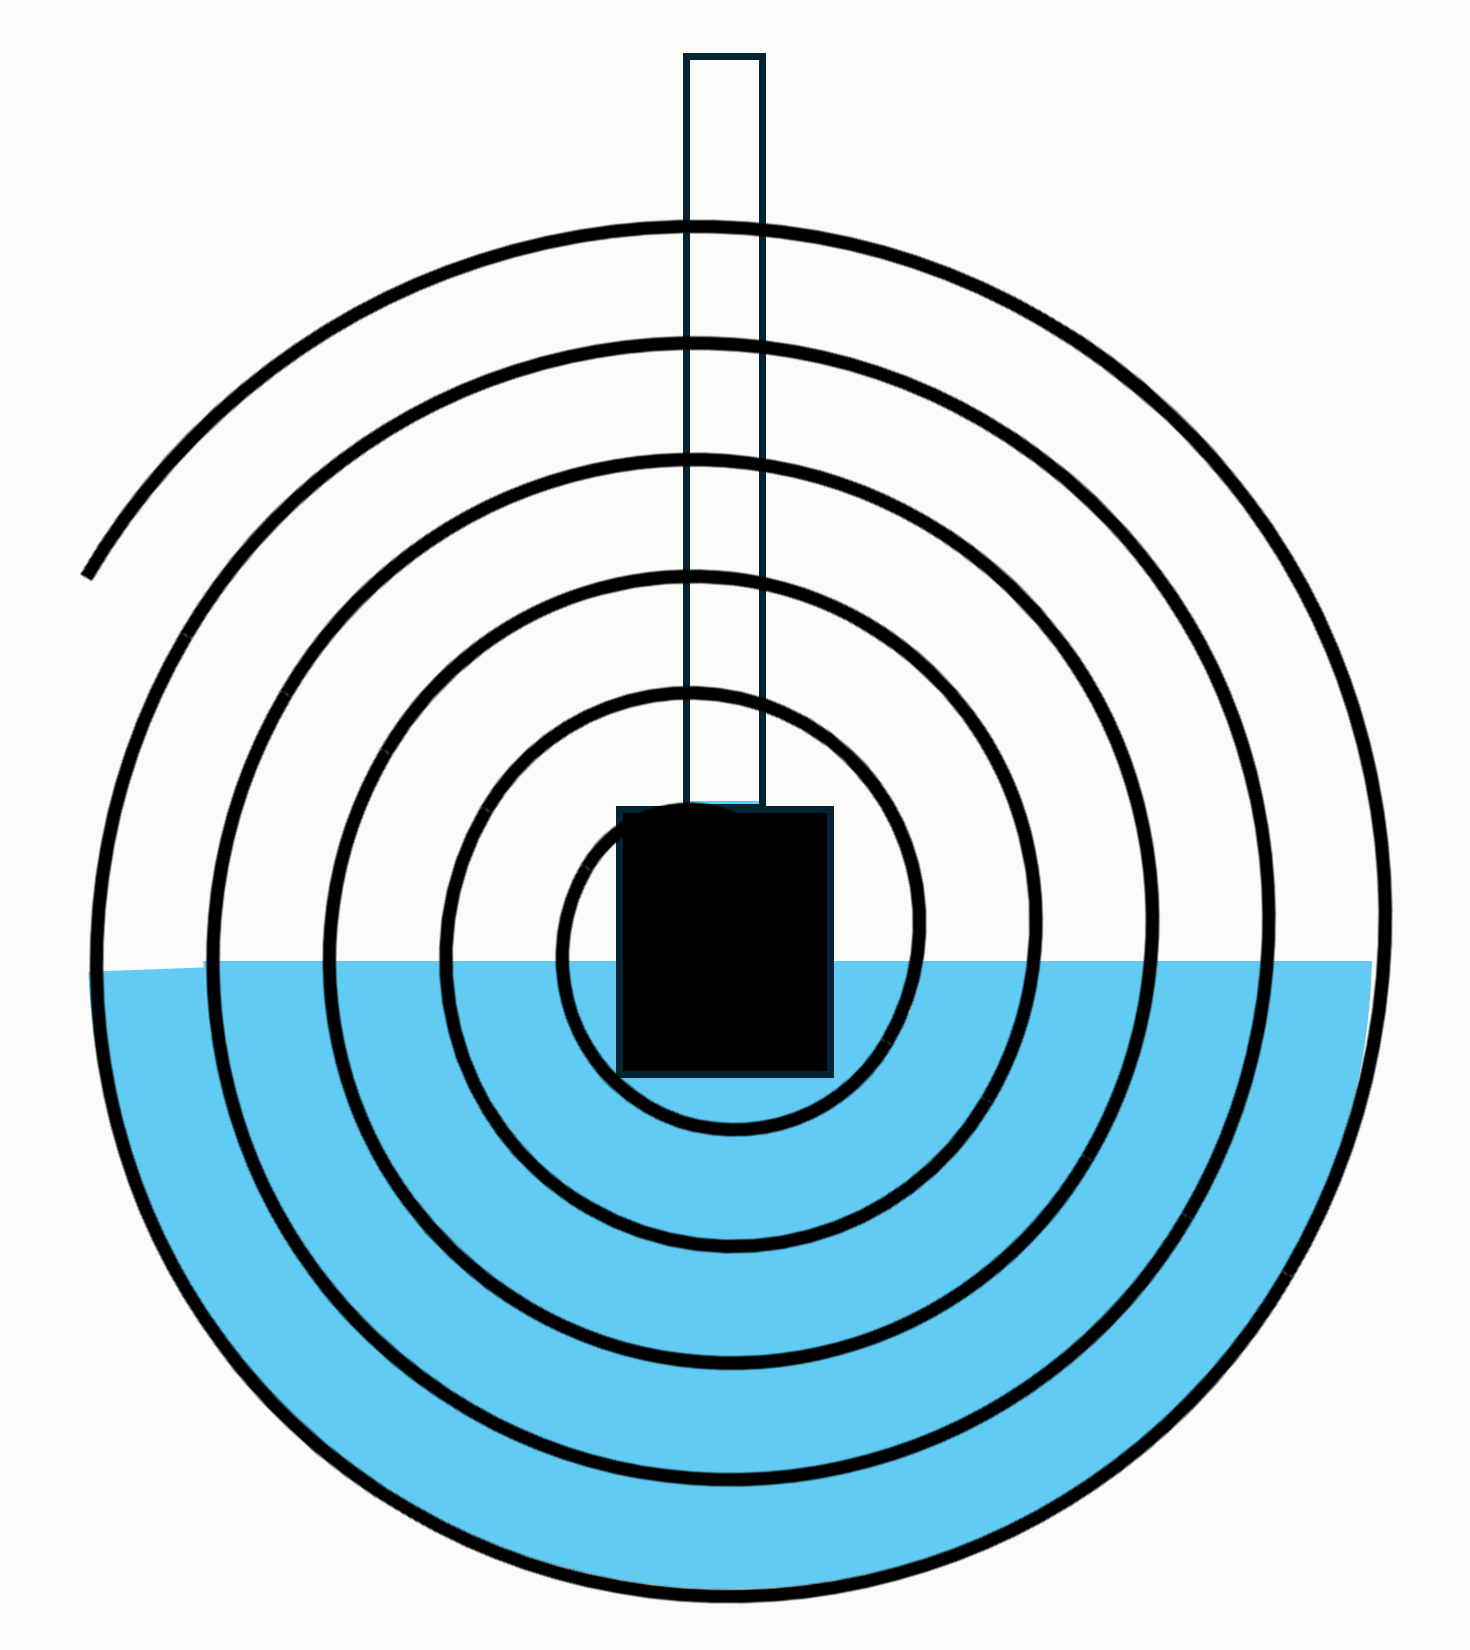
\includegraphics[width=0.6\columnwidth]{pockets_schematic.png}
  \caption{Esquema da espiral com tampões de água (azul) e bolsões de ar. O centro está ligado ao tubo vertical de recalque.}
  \label{fig:pockets}
\end{figure}

%=====================================================================
\section{Arranjo experimental}
\label{sec:setup}
%=====================================================================

A bomba (Fig.~\ref{fig:setup}) consiste em um tubo de silicone enrolado em espiral sobre um disco de acrílico, um suporte impresso em 3D, uma junta rotativa e um tubo vertical de recalque, e é acionada por uma furadeira elétrica. Os experimentos foram feitos em uma piscina de \SI{500}{L}, para que o nível da água não mudasse significativamente durante uma medida.

\begin{figure}[t]
  \centering
  \begin{subfigure}[b]{0.49\columnwidth}\centering
    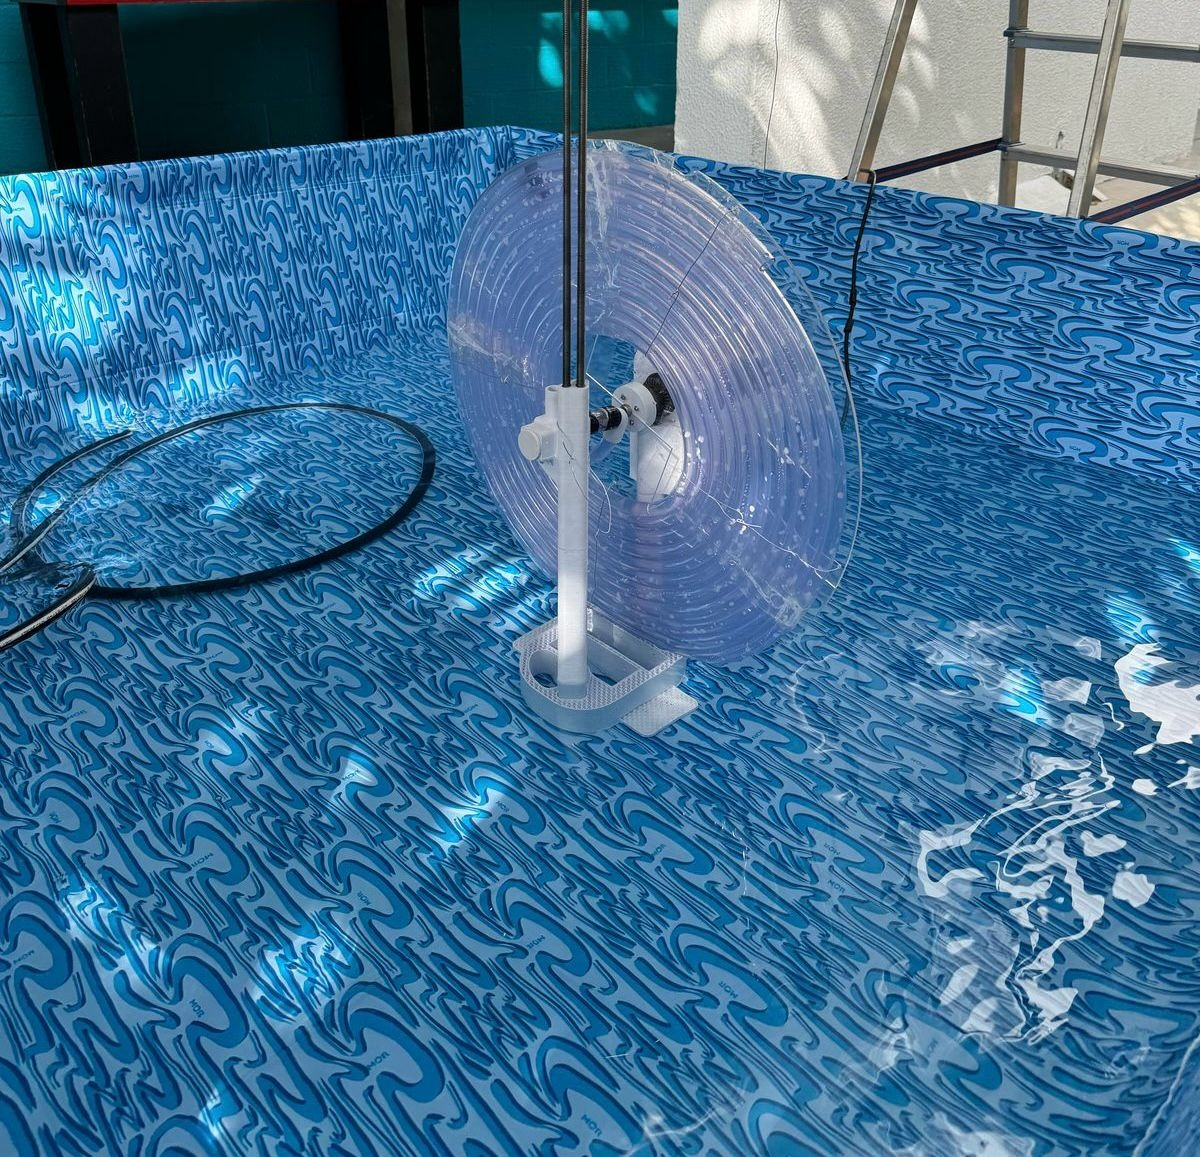
\includegraphics[width=\linewidth,height=3.3cm,keepaspectratio]{pump_photo.jpg}\caption{}\end{subfigure}\hfill
  \begin{subfigure}[b]{0.49\columnwidth}\centering
    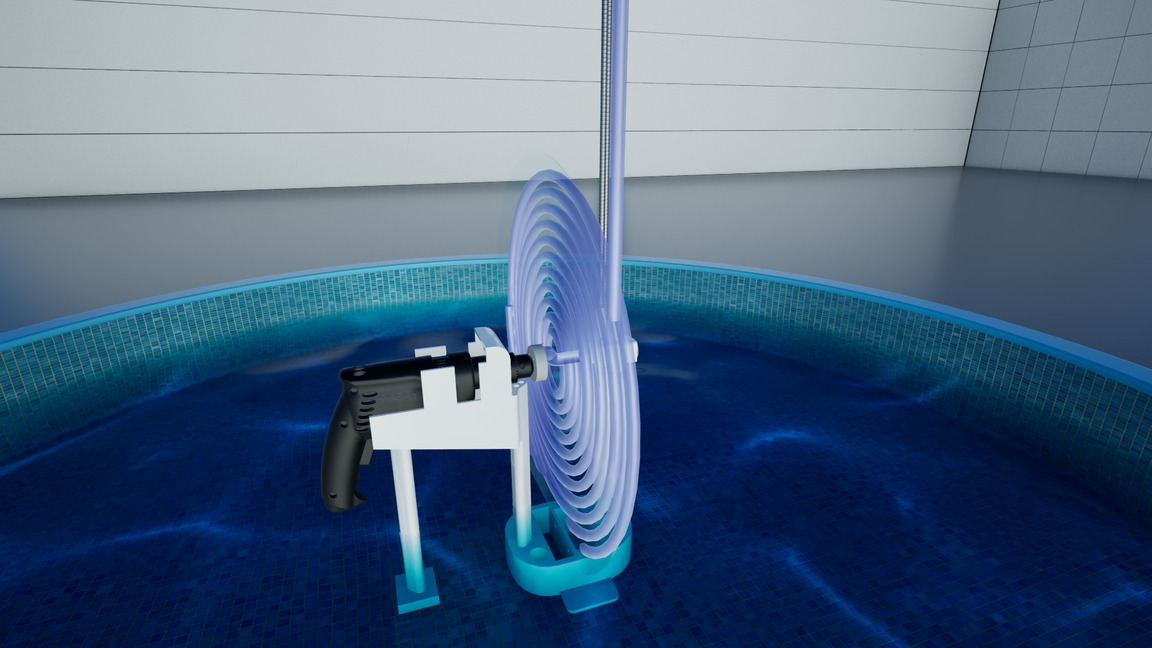
\includegraphics[width=\linewidth,height=3.3cm,keepaspectratio]{setup_render.jpg}\caption{}\end{subfigure}\\[2pt]
  \begin{subfigure}[b]{\columnwidth}\centering
    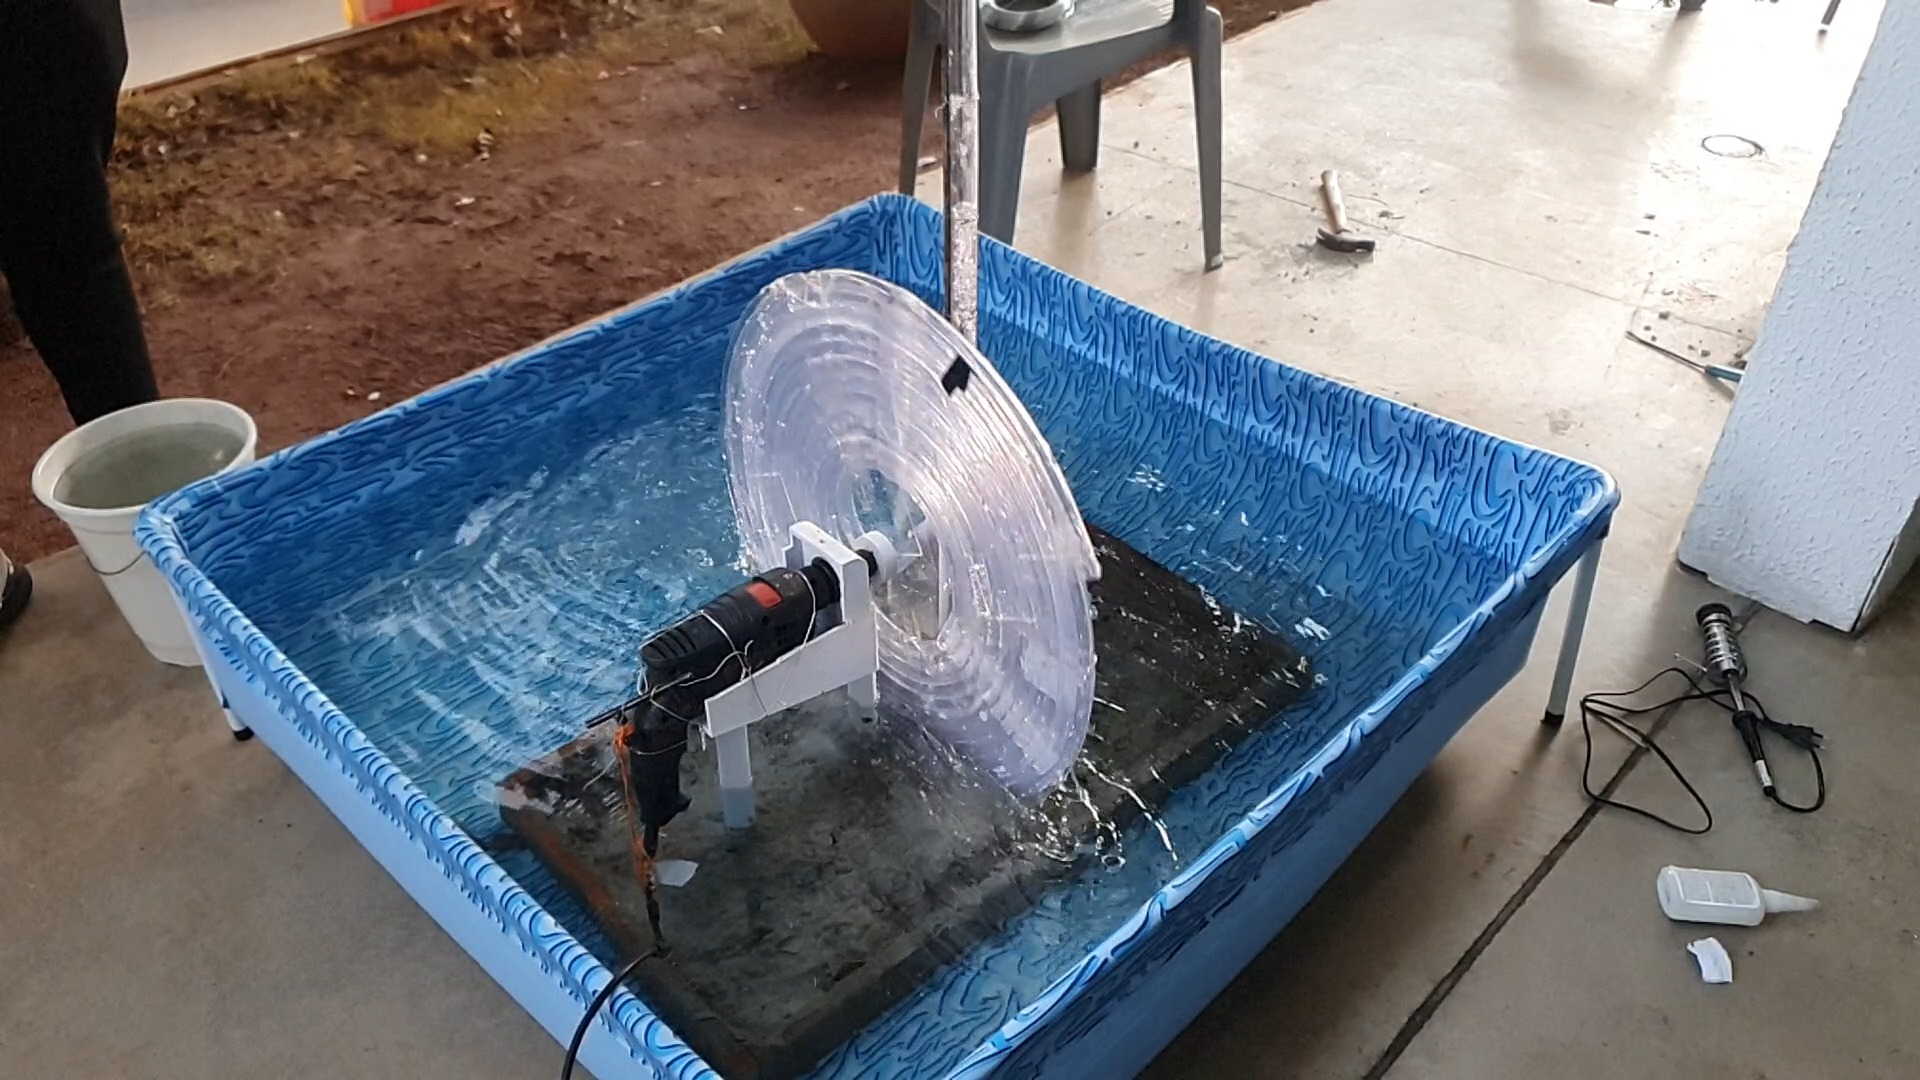
\includegraphics[width=0.8\linewidth]{setup_pool.jpg}\caption{}\end{subfigure}
  \caption{(a)~Bomba de Wirtz em operação. (b)~Modelo CAD da bomba, do suporte e da furadeira. (c)~Arranjo na piscina de \SI{500}{L}.}
  \label{fig:setup}
\end{figure}

\paragraph*{Suporte e tubo de recalque.} O suporte foi projetado em CAD, impresso em 3D em PLA e enrijecido com barras de aço de cada lado. Um tubo vertical de \SI{2}{m} foi fixado a ele e ligado à espiral por uma junta rotativa. O tubo foi marcado a cada \SI{10}{cm} a partir do ponto de conexão, e a altura da água foi medida em vídeo com o software Tracker, usando essas marcas como referência [Fig.~\ref{fig:support}(a)]. A base era originalmente oca, para ser preenchida com água e ganhar estabilidade, mas oscilava fortemente durante a operação; fixá-la em um bloco de concreto reduziu drasticamente as oscilações [Fig.~\ref{fig:support}(b,c)].

\begin{figure}[t]
  \centering
  \begin{subfigure}[b]{0.25\columnwidth}\centering
    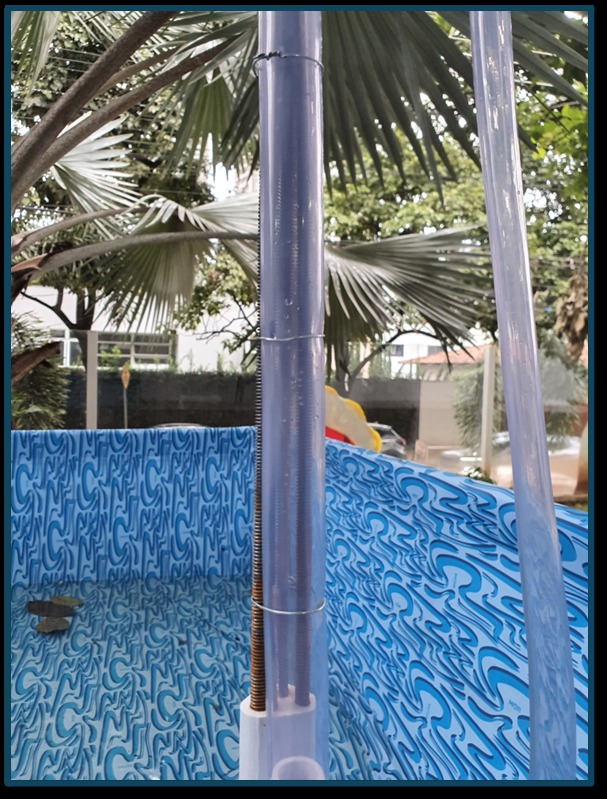
\includegraphics[width=\linewidth,height=3.6cm,keepaspectratio]{tube_markings.jpg}\caption{}\end{subfigure}\hfill
  \begin{subfigure}[b]{0.25\columnwidth}\centering
    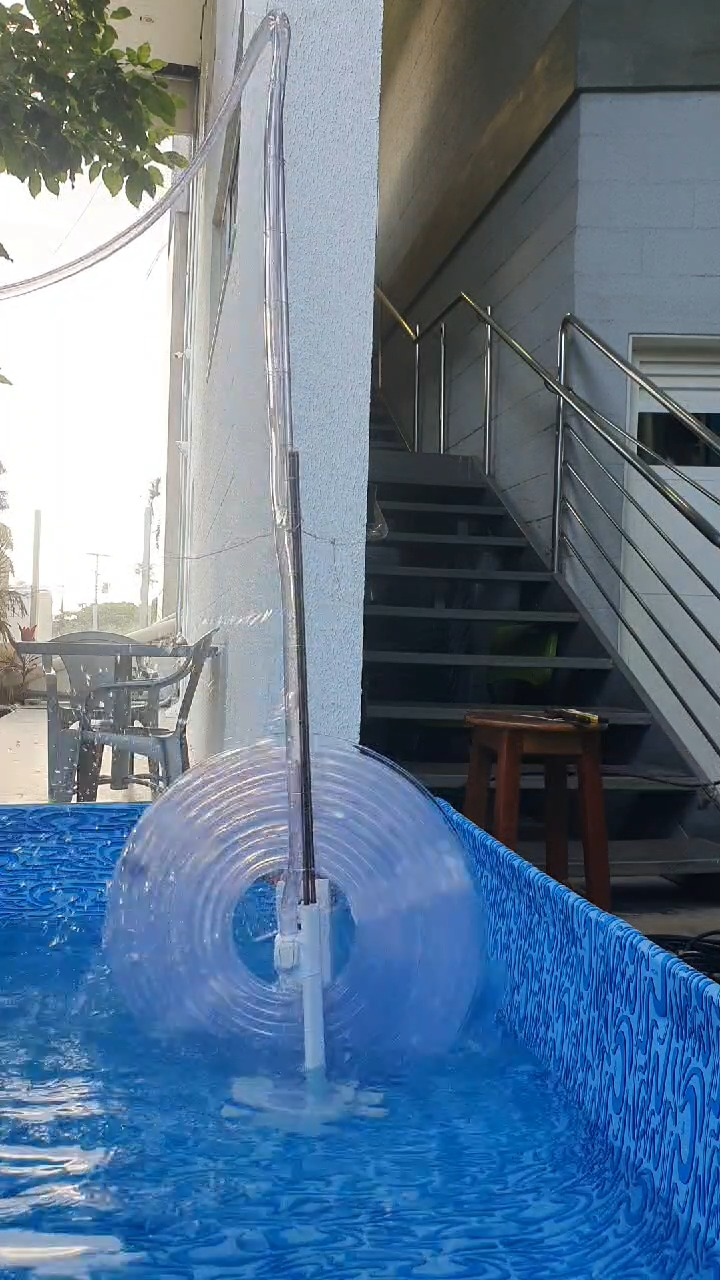
\includegraphics[width=\linewidth,height=3.6cm,keepaspectratio]{support_original.jpg}\caption{}\end{subfigure}\hfill
  \begin{subfigure}[b]{0.44\columnwidth}\centering
    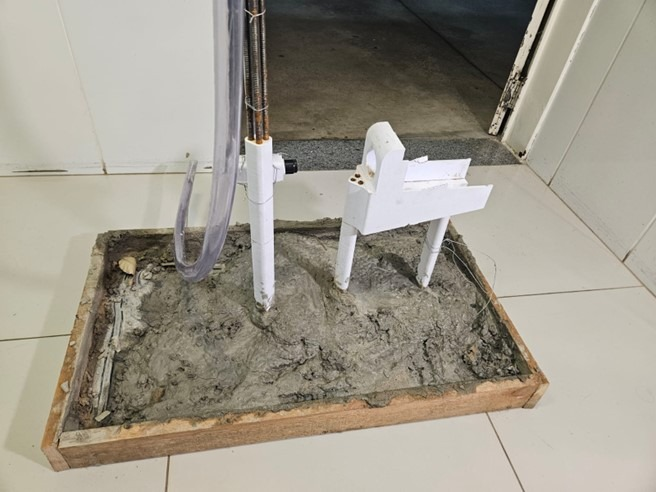
\includegraphics[width=\linewidth,height=3.6cm,keepaspectratio]{concrete_base.jpg}\caption{}\end{subfigure}
  \caption{(a)~Tubo de recalque com marcas a cada \SI{10}{cm}. (b)~Base oca original, que oscilava durante a operação. (c)~Suporte fixado em concreto.}
  \label{fig:support}
\end{figure}

\paragraph*{Junta rotativa.} Uma junta rotativa liga a espiral em rotação ao tubo de recalque estático sem vazamento significativo e sem torcer os tubos. Juntas comerciais usam vedações de borracha, uma extremidade oca e construção metálica [Fig.~\ref{fig:joint}(a)]; projetamos e imprimimos em 3D uma junta de PLA, integrada ao suporte da bomba, com furos laterais para a passagem da água [Fig.~\ref{fig:joint}(b)].

\begin{figure}[t]
  \centering
  \begin{subfigure}[b]{0.45\columnwidth}\centering
    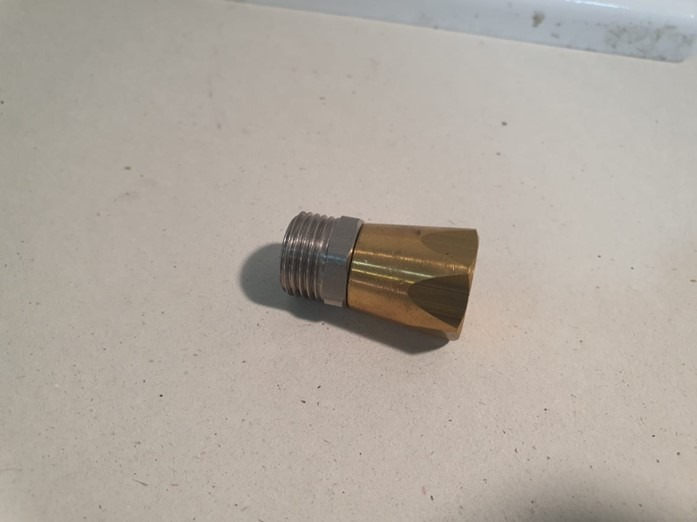
\includegraphics[width=\linewidth]{joint_store.jpg}\caption{}\end{subfigure}\hfill
  \begin{subfigure}[b]{0.52\columnwidth}\centering
    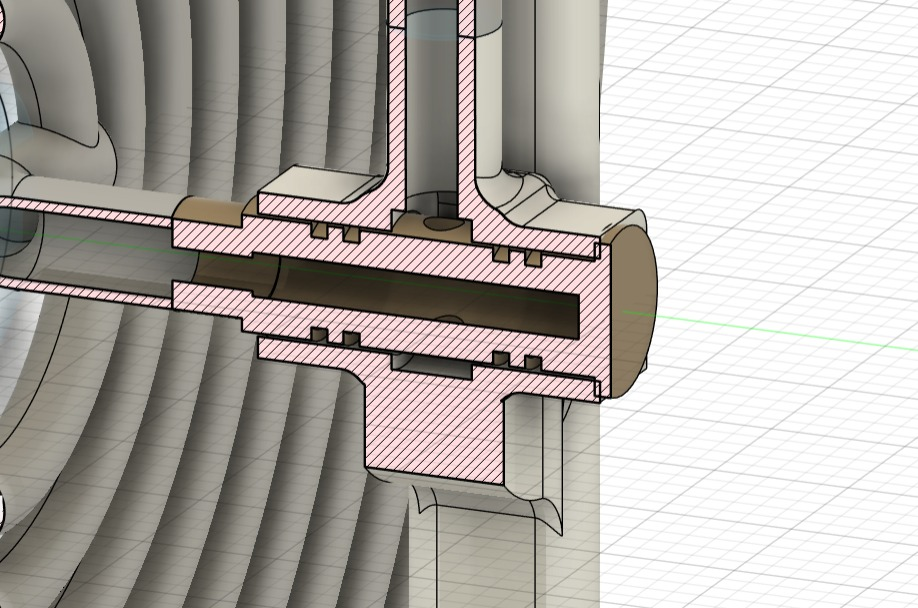
\includegraphics[width=\linewidth]{joint_printed.jpg}\caption{}\end{subfigure}
  \caption{(a)~Junta rotativa comercial. (b)~Corte da junta rotativa impressa em 3D.}
  \label{fig:joint}
\end{figure}

\paragraph*{Espiral e acionamento.} A espiral foi feita amarrando um tubo de silicone com arame metálico através de furos em um disco de acrílico cortado a laser (Fig.~\ref{fig:spiral}). Uma marca de alto contraste no disco foi usada para medir a velocidade angular com o Tracker. A bomba foi acionada por uma furadeira elétrica Bosch, que fornece torque suficiente; com o gatilho totalmente pressionado, a velocidade angular é $\omega=(450\pm5)$~rpm.

\begin{figure}[t]
  \centering
  \begin{subfigure}[b]{0.32\columnwidth}\centering
    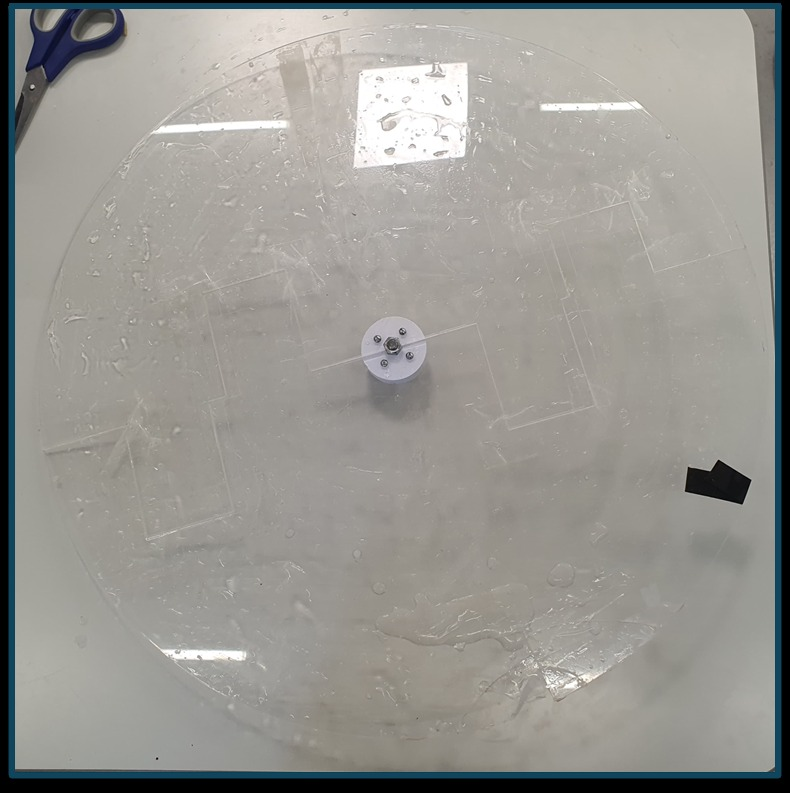
\includegraphics[width=\linewidth]{acrylic_disk.jpg}\caption{}\end{subfigure}\hfill
  \begin{subfigure}[b]{0.32\columnwidth}\centering
    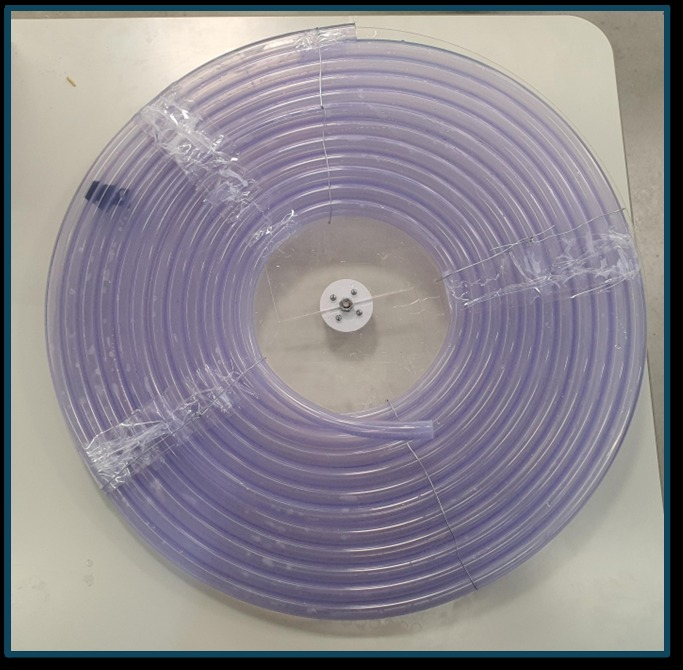
\includegraphics[width=\linewidth]{spiral_mounted.jpg}\caption{}\end{subfigure}\hfill
  \begin{subfigure}[b]{0.32\columnwidth}\centering
    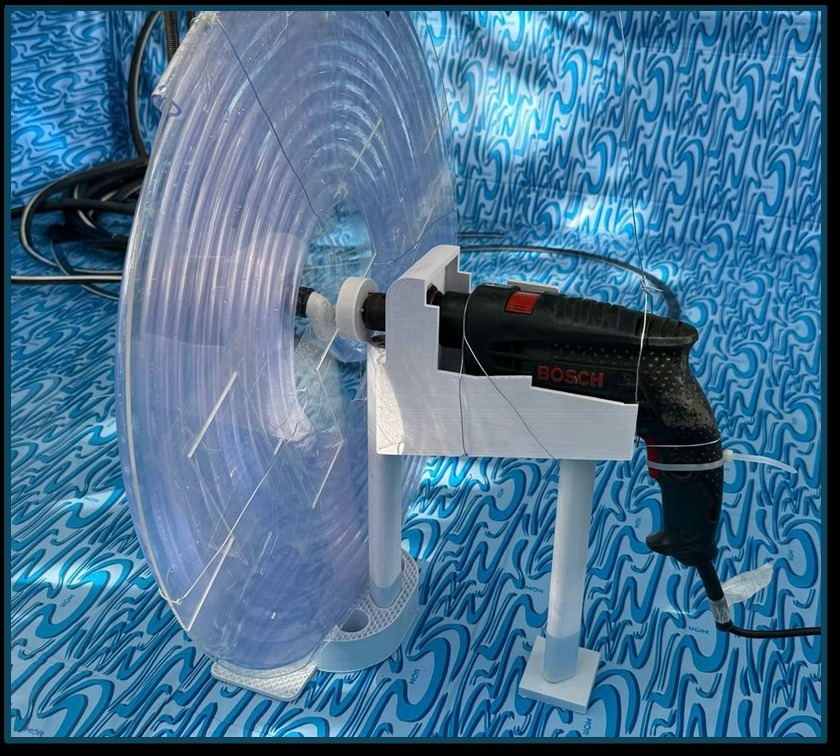
\includegraphics[width=\linewidth]{drill_mount.jpg}\caption{}\end{subfigure}
  \caption{(a)~Disco de acrílico cortado a laser com a marca de alto contraste usada para o rastreamento. (b)~Tubo de silicone amarrado ao disco. (c)~Furadeira montada no suporte.}
  \label{fig:spiral}
\end{figure}

\paragraph*{Parâmetros.} A profundidade de imersão da entrada, a rotação e o tubo foram variados conforme a Tabela~\ref{tab:params}. Foram usados três tubos de silicone (tubos~1--3) de diâmetros internos diferentes, cobrindo a faixa da Tabela~\ref{tab:params}, e foram construídas espirais com $N=4$ e $N=12$ voltas. A altura de bombeamento $h$ é medida a partir da superfície livre da piscina. Como o eixo de rotação, onde começa o tubo de recalque, fica acima dessa superfície, podem ser lidas alturas ligeiramente maiores que o comprimento de \SI{2}{m} do tubo graduado.

\begin{table}[b]
  \caption{Parâmetros experimentais.}
  \label{tab:params}
  \begin{ruledtabular}
  \begin{tabular}{lc}
    Parâmetro & Valores \\
    \midrule
    Imersão $d$ ($\pm\SI{0.05}{cm}$) & 4,00; 6,00; \ldots; 18,00 \\
    Rotação $\omega$ ($\pm\SI{5}{rpm}$) & 100; 200; 300; 400; 450 \\
    Diâmetro $D$ ($\pm\SI{0.05}{cm}$) & 1,50; 2,00; 3,00 \\
  \end{tabular}
  \end{ruledtabular}
\end{table}

%=====================================================================
\section{Modelo teórico}
\label{sec:theory}
%=====================================================================

\subsection{Espiral desenrolada e geometria de Arquimedes}

Analisamos o tubo como se fosse desenrolado em um canal reto com uma coordenada $x$ ao longo de seu eixo (Fig.~\ref{fig:unrolled}). Isso reduz o problema de duas coordenadas para uma, torna explícita a disposição dos tampões e permite explorar a periodicidade da espiral.

\begin{figure}[t]
  \centering
  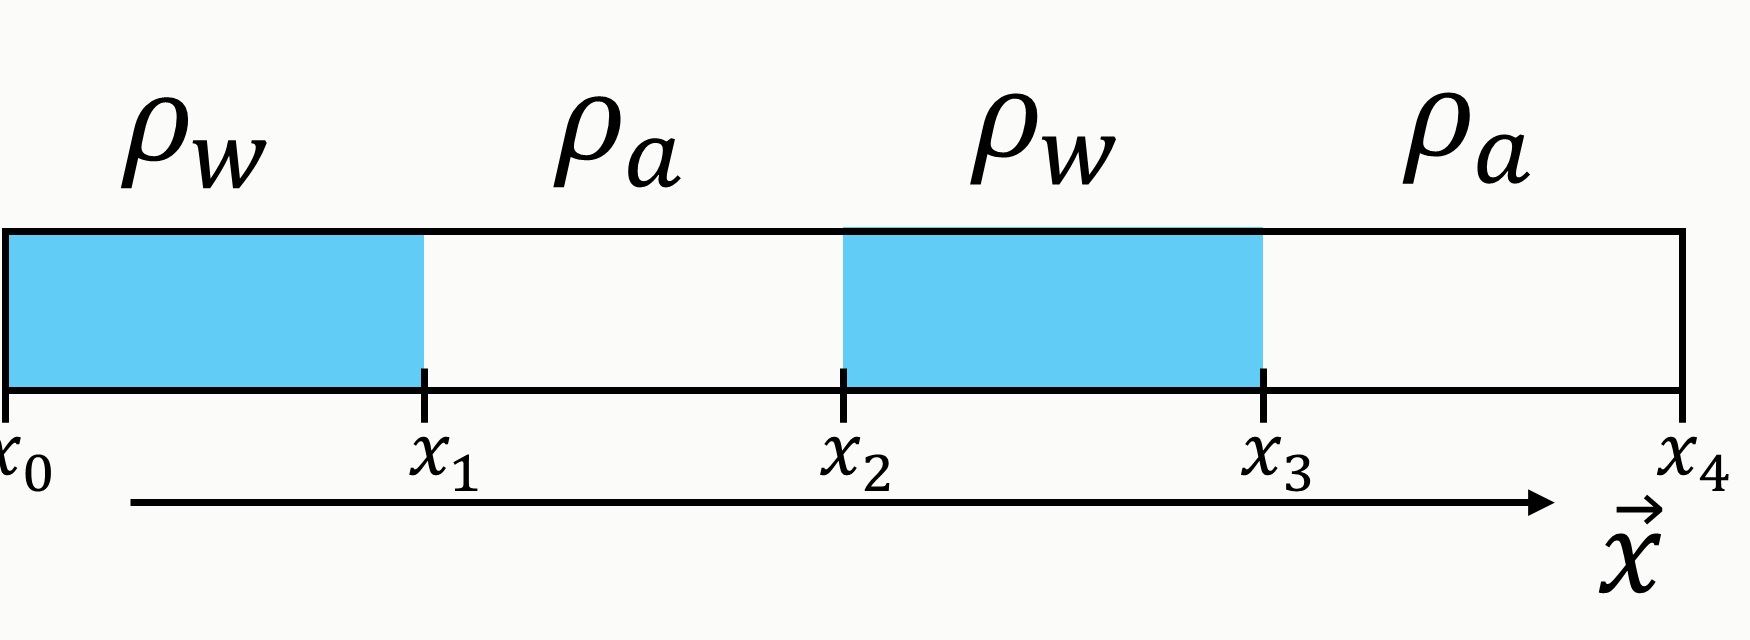
\includegraphics[width=0.9\columnwidth]{unrolled_tube.png}
  \caption{A espiral desenrolada em um canal unidimensional, com regiões alternadas de água ($\rho_w$, azul) e de ar ($\rho_a$).}
  \label{fig:unrolled}
\end{figure}

A espiral é uma espiral de Arquimedes de passo $\varepsilon$ (a distância radial entre voltas consecutivas),
\begin{equation}
  r = \frac{\varepsilon\theta}{2\pi}, \qquad 0\le\theta\le\theta_{\max}=2\pi N .
\end{equation}
O elemento de arco é $ds=\sqrt{r^2+(dr/d\theta)^2}\,d\theta=(\varepsilon/2\pi)\sqrt{1+\theta^2}\,d\theta$, cuja integral é exata (Fig.~\ref{fig:spiral_param}):
\begin{equation}
  s(\theta) = \frac{\varepsilon}{4\pi}\left[\theta\sqrt{1+\theta^2} + \operatorname{arsinh}\theta\right]
  = \frac{\varepsilon\theta^2}{4\pi}\left[1+O\!\left(\frac{\ln\theta}{\theta^2}\right)\right].
  \label{eq:arc}
\end{equation}
Medindo $x$ a partir da entrada (a extremidade externa) em direção ao centro,
\begin{equation}
  x(\theta) = \frac{\varepsilon}{4\pi}\left(\theta_{\max}^2-\theta^2\right), \qquad
  L = \frac{\varepsilon\theta_{\max}^2}{4\pi} = \pi\varepsilon N^2 \simeq \pi R_oN,
  \label{eq:xtheta}
\end{equation}
onde $L$ é o comprimento do tubo e $R_o=\varepsilon N$ o raio externo: o tubo tem o comprimento de $N$ circunferências de raio médio $R_o/2$. A espiral cruza cada círculo $r=$~const sob o ângulo de passo $\alpha$, com
\begin{equation}
  \tan\alpha = \frac{1}{\theta}, \qquad \frac{dr}{ds} = \sin\alpha = \frac{1}{\sqrt{1+\theta^2}} \simeq \frac{\varepsilon}{2\pi r},
  \label{eq:pitch}
\end{equation}
que é a razão entre o passo e a circunferência local.

\begin{figure}[t]
  \centering
  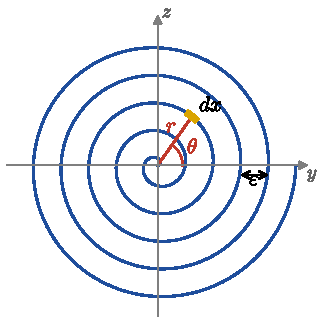
\includegraphics[width=0.7\columnwidth]{spiral_param.pdf}
  \caption{Espiral de Arquimedes $r=\varepsilon\theta/2\pi$ no plano da bomba, mostrando o passo $\varepsilon$, as coordenadas polares $(r,\theta)$ e o elemento de arco $dx$ ao longo do tubo.}
  \label{fig:spiral_param}
\end{figure}

\subsection{Funções indicadoras e notação matricial}

A presença de duas fases é descrita pelas funções indicadoras $I_k(\bm r,t)$, $k\in\{w,a\}$, iguais a 1 na fase $k$ e 0 fora dela~\cite{drew1983,ishii2011}. Para escrever uma \emph{única} equação válida em todo o escoamento, em vez de uma equação por fase, reunimos as propriedades das fases em vetores linha e as funções indicadoras em um vetor coluna,
\begin{equation}
  \bm\rho = \begin{pmatrix}\rho_w & \rho_a\end{pmatrix}, \qquad
  \bm\mu = \begin{pmatrix}\mu_w & \mu_a\end{pmatrix}, \qquad
  \mathbf I = \begin{pmatrix} I_w\\ I_a\end{pmatrix},
  \label{eq:matrices}
\end{equation}
de modo que o produto matricial $(1\times2)(2\times1)$ fornece a propriedade local da mistura:
\begin{align}
  \bm\rho\mathbf I &= \rho_wI_w + \rho_aI_a
  = \begin{cases}\rho_w, & \bm r\in\dV_w,\\ \rho_a, & \bm r\in\dV_a,\end{cases} \nonumber\\
  \bm\mu\mathbf I &= \mu_wI_w+\mu_aI_a .
  \label{eq:rhoI}
\end{align}
Essa notação é mais do que uma abreviação. As funções indicadoras formam uma partição da unidade por projetores ortogonais,
\begin{equation}
  I_kI_l = \delta_{kl}\,I_k, \qquad I_w + I_a = 1,
  \label{eq:projectors}
\end{equation}
e por isso qualquer função de uma propriedade da mistura atua componente a componente, $f(\bm\rho\mathbf I)=f(\bm\rho)\,\mathbf I$, com $f(\bm\rho)=\big(f(\rho_w)\ \ f(\rho_a)\big)$. Por exemplo, a viscosidade cinemática local é $(\bm\mu\mathbf I)/(\bm\rho\mathbf I)=\big(\nu_w\ \ \nu_a\big)\mathbf I$.

As funções indicadoras são transportadas pelas interfaces, que se movem com velocidade $\bm u_i$, e seus gradientes são distribuições concentradas nas interfaces:
\begin{equation}
  \frac{\partial \mathbf I}{\partial t} + \bm u_i\cdot\nabla \mathbf I = 0, \qquad
  \nabla I_k = -\,\bm n_k\,\delta_i ,
  \label{eq:topological}
\end{equation}
onde $\bm n_k$ é a normal que aponta para fora da fase $k$ e $\delta_i$ a delta de superfície. No canal desenrolado, o tampão $j$ ocupa o intervalo $[a_j,b_j]$, e
\begin{align}
  I_w(x) &= \sum_{j}\left[H(x-a_j)-H(x-b_j)\right], \nonumber\\
  \frac{dI_w}{dx} &= -\frac{dI_a}{dx} = \sum_j\left[\delta(x-a_j)-\delta(x-b_j)\right],
  \label{eq:Iw}
\end{align}
com $H$ a função de Heaviside.

\paragraph*{Médias.} Seja $\gamma$ a grandeza cuja média se deseja tomar, por exemplo a velocidade $w$. A média volumétrica de $\gamma$ na fase $k$ é definida pela integral~\cite{whitaker1999}
\begin{equation}
  \avg{\gamma}_k = \frac{1}{\dV}\int_\dV I_k(\bm r)\,\gamma(\bm r)\,d\dV
  = \frac1L\int_0^L I_k(x)\,\gamma(x)\,dx,
  \label{eq:avg}
\end{equation}
onde a segunda forma vale para um canal de seção constante. A função indicadora aparece apenas \emph{dentro da integral que define a média}: ela não é a grandeza média, mas o seletor que restringe a integração à fase $k$, e o índice $k$ do colchete registra essa escolha. Reunindo as duas fases em um vetor coluna,
\begin{align}
  \avg{\gamma} &\equiv \begin{pmatrix}\avg{\gamma}_w\\ \avg{\gamma}_a\end{pmatrix}, \nonumber\\
  \bm\rho\avg{\gamma} &= \rho_w\avg{\gamma}_w + \rho_a\avg{\gamma}_a = \sum_k\rho_k\avg{\gamma}_k ,
  \label{eq:avgvec}
\end{align}
as somas sobre as fases tornam-se o mesmo produto matricial $(1\times2)(2\times1)$ da Eq.~\eqref{eq:rhoI}. Com $\gamma=1$ obtêm-se as frações volumétricas, $\bm\alpha=\avg{1}=(\alpha_w,\alpha_a)^{\mathsf T}$, com $\alpha_w+\alpha_a=1$, e a densidade média da mistura é $\bar\rho=\bm\rho\bm\alpha$. Integrando sobre $\dV$ a identidade pontual $I_k\nabla\gamma=\nabla(I_k\gamma)-\gamma\nabla I_k$ e usando a Eq.~\eqref{eq:topological}, obtém-se o teorema da média espacial,
\begin{equation}
  \avg{\nabla\gamma}_k = \nabla\avg{\gamma}_k + \frac{1}{\dV}\int_{A_i}\gamma\,\bm n_k\,dA ,
  \label{eq:averaging_theorem}
\end{equation}
cuja integral sobre as interfaces será a origem física do bombeamento.

\paragraph*{Continuidade.} Na notação matricial, a conservação da massa é $\partial_t(\bm\rho\mathbf I)+\partial_x(\bm\rho\mathbf I\,w)=0$. Expandindo a derivada do produto e usando a Eq.~\eqref{eq:topological} com $\bm u_i=w$,
\begin{align}
  (\bm\rho\mathbf I)\,\frac{\partial w}{\partial x}
  &= -\,\bm\rho\left(\frac{\partial\mathbf I}{\partial t}+w\frac{\partial\mathbf I}{\partial x}\right)
  - \mathbf I^{\mathsf T}\!\left(\frac{\partial\bm\rho^{\mathsf T}}{\partial t}+w\frac{\partial\bm\rho^{\mathsf T}}{\partial x}\right) \nonumber\\
  &= -\,I_a\,\frac{D\rho_a}{Dt},
  \label{eq:continuity}
\end{align}
pois $\rho_w$ é constante. Dentro de cada tampão, portanto, $\partial_xw=0$: os tampões se movem como blocos rígidos, e a velocidade só pode variar de um tampão para o seguinte, o que é acomodado pela compressão dos bolsões de ar.

\subsection{Navier--Stokes no referencial da espiral}

Escrevemos o balanço de momento no referencial que gira com a espiral à velocidade angular $\omega$, no qual o tubo está em repouso. Nesse referencial não inercial, o fluido está sujeito, além da pressão, da gravidade e das forças viscosas, à força centrífuga $\rho\,\omega^2\bm r$ e à força de Coriolis $-2\rho\,\bm\omega\times\bm w$, onde $\bm w$ é a velocidade relativa ao tubo. Para um escoamento unidimensional, $\bm w=w\,\hat{\bm t}$, com $\hat{\bm t}$ a tangente ao tubo, e a força de Coriolis é perpendicular ao tubo: ela gera apenas um escoamento secundário na seção e não entra no balanço axial. A força centrífuga deriva do potencial
\begin{equation}
  \Phi_c = \tfrac12\,\omega^2r^2, \qquad \rho\,\omega^2\bm r\cdot\hat{\bm t} = \rho\,\frac{\partial\Phi_c}{\partial x}.
\end{equation}
Com a notação~\eqref{eq:rhoI}, a equação de Navier--Stokes unidimensional para todo o escoamento bifásico é
\begin{multline}
  (\bm\rho\mathbf I)\left(\frac{\partial w}{\partial t}+w\frac{\partial w}{\partial x}\right)
  = -\frac{\partial P}{\partial x}
  + (\bm\rho\mathbf I)\left(g_x+\frac{\partial\Phi_c}{\partial x}\right) \\
  + (\bm\mu\mathbf I)\,\frac{\partial^2w}{\partial x^2}
  - \frac{4\tau_w}{D}\,I_w ,
  \label{eq:momentum}
\end{multline}
onde $g_x$ é a componente da gravidade ao longo do tubo, $\tau_w$ a tensão de cisalhamento na parede sobre os tampões e $D$ o diâmetro interno do tubo. No laboratório, a configuração dos tampões é estacionária; no referencial da espiral, ela é periódica, e a aceleração material de cada tampão é $w\,\partial_xw$ ao longo do campo de velocidades $w(x)$ que os tampões assumem em cada posição do tubo. Integrando a Eq.~\eqref{eq:momentum} ao longo do canal e dividindo por $L$, cada produto $(\bm\rho\mathbf I)\gamma=\sum_k\rho_kI_k\gamma$ se torna, pela definição~\eqref{eq:avg}, o produto $\bm\rho\avg{\gamma}$ da Eq.~\eqref{eq:avgvec}; o termo de parede, que contém apenas $I_w$, torna-se uma média sobre a água. Obtemos a equação mestra do modelo:
\begin{multline}
  \frac{P(L)-P(0)}{L}
  = \underbrace{\bm\rho\avg{\partial_x\Phi_c}}_{\text{centrífugo}}
  - \underbrace{\bm\rho\avg{w\,\partial_xw}}_{\text{inercial}}
  + \underbrace{\bm\rho\avg{g_x}}_{\text{gravitacional}} \\
  + \underbrace{\bm\mu\avg{\partial_x^2w}}_{\text{viscoso axial}}
  - \underbrace{\frac{4}{D}\avg{\tau_w}_w}_{\text{parede}} .
  \label{eq:averaged}
\end{multline}
Cada um dos cinco termos é um produto $(1\times2)(2\times1)$ que soma as contribuições da água e do ar. A seguir, avaliamos todos explicitamente com a parametrização da espiral.

\subsection{Parametrização ao longo do tubo}

Com $x$ medido a partir da entrada e a forma assintótica da Eq.~\eqref{eq:arc}, $x=(\varepsilon/4\pi)(\theta_{\max}^2-\theta^2)$, todas as grandezas cinemáticas tornam-se funções explícitas de $x$:
\begin{align}
  \theta(x) &= \sqrt{\frac{4\pi}{\varepsilon}(L-x)}, \qquad
  r(x) = \frac{\varepsilon\theta}{2\pi} = \sqrt{\frac{\varepsilon}{\pi}(L-x)}, \label{eq:param_r}\\
  w(x) &= \omega r(x) = \omega\sqrt{\frac{\varepsilon}{\pi}(L-x)}, \label{eq:param_w}\\
  \Phi_c(x) &= \tfrac12\omega^2r^2 = \frac{\omega^2\varepsilon}{2\pi}(L-x), \label{eq:param_phi}\\
  g_x(x,t) &= g\cos\!\big(\theta(x)+\omega t\big). \label{eq:param_g}
\end{align}
A velocidade relativa $w=\omega r$ expressa que um tampão permanece praticamente parado no laboratório enquanto o tubo desliza sob ele (Fig.~\ref{fig:frames}): ele avança uma volta para dentro a cada revolução. A Eq.~\eqref{eq:param_g} é a gravidade vista do referencial em rotação, onde ela gira com $-\omega$; o ângulo $\phi=\theta+\omega t$ é o ângulo do elemento de tubo no laboratório, escolhido de modo que $\phi=0$ corresponda a um trecho de tubo vertical. Para $\omega t=0$ ela se reduz a $g\cos\theta$. Usaremos também
\begin{equation}
  \frac{dr}{dx} = -\frac{\varepsilon}{2\pi r}, \qquad dx = -\frac{\varepsilon}{2\pi}\,\theta\,d\theta .
  \label{eq:drdx}
\end{equation}

\begin{figure}[t]
  \centering
  \begin{subfigure}[b]{0.49\columnwidth}\centering
    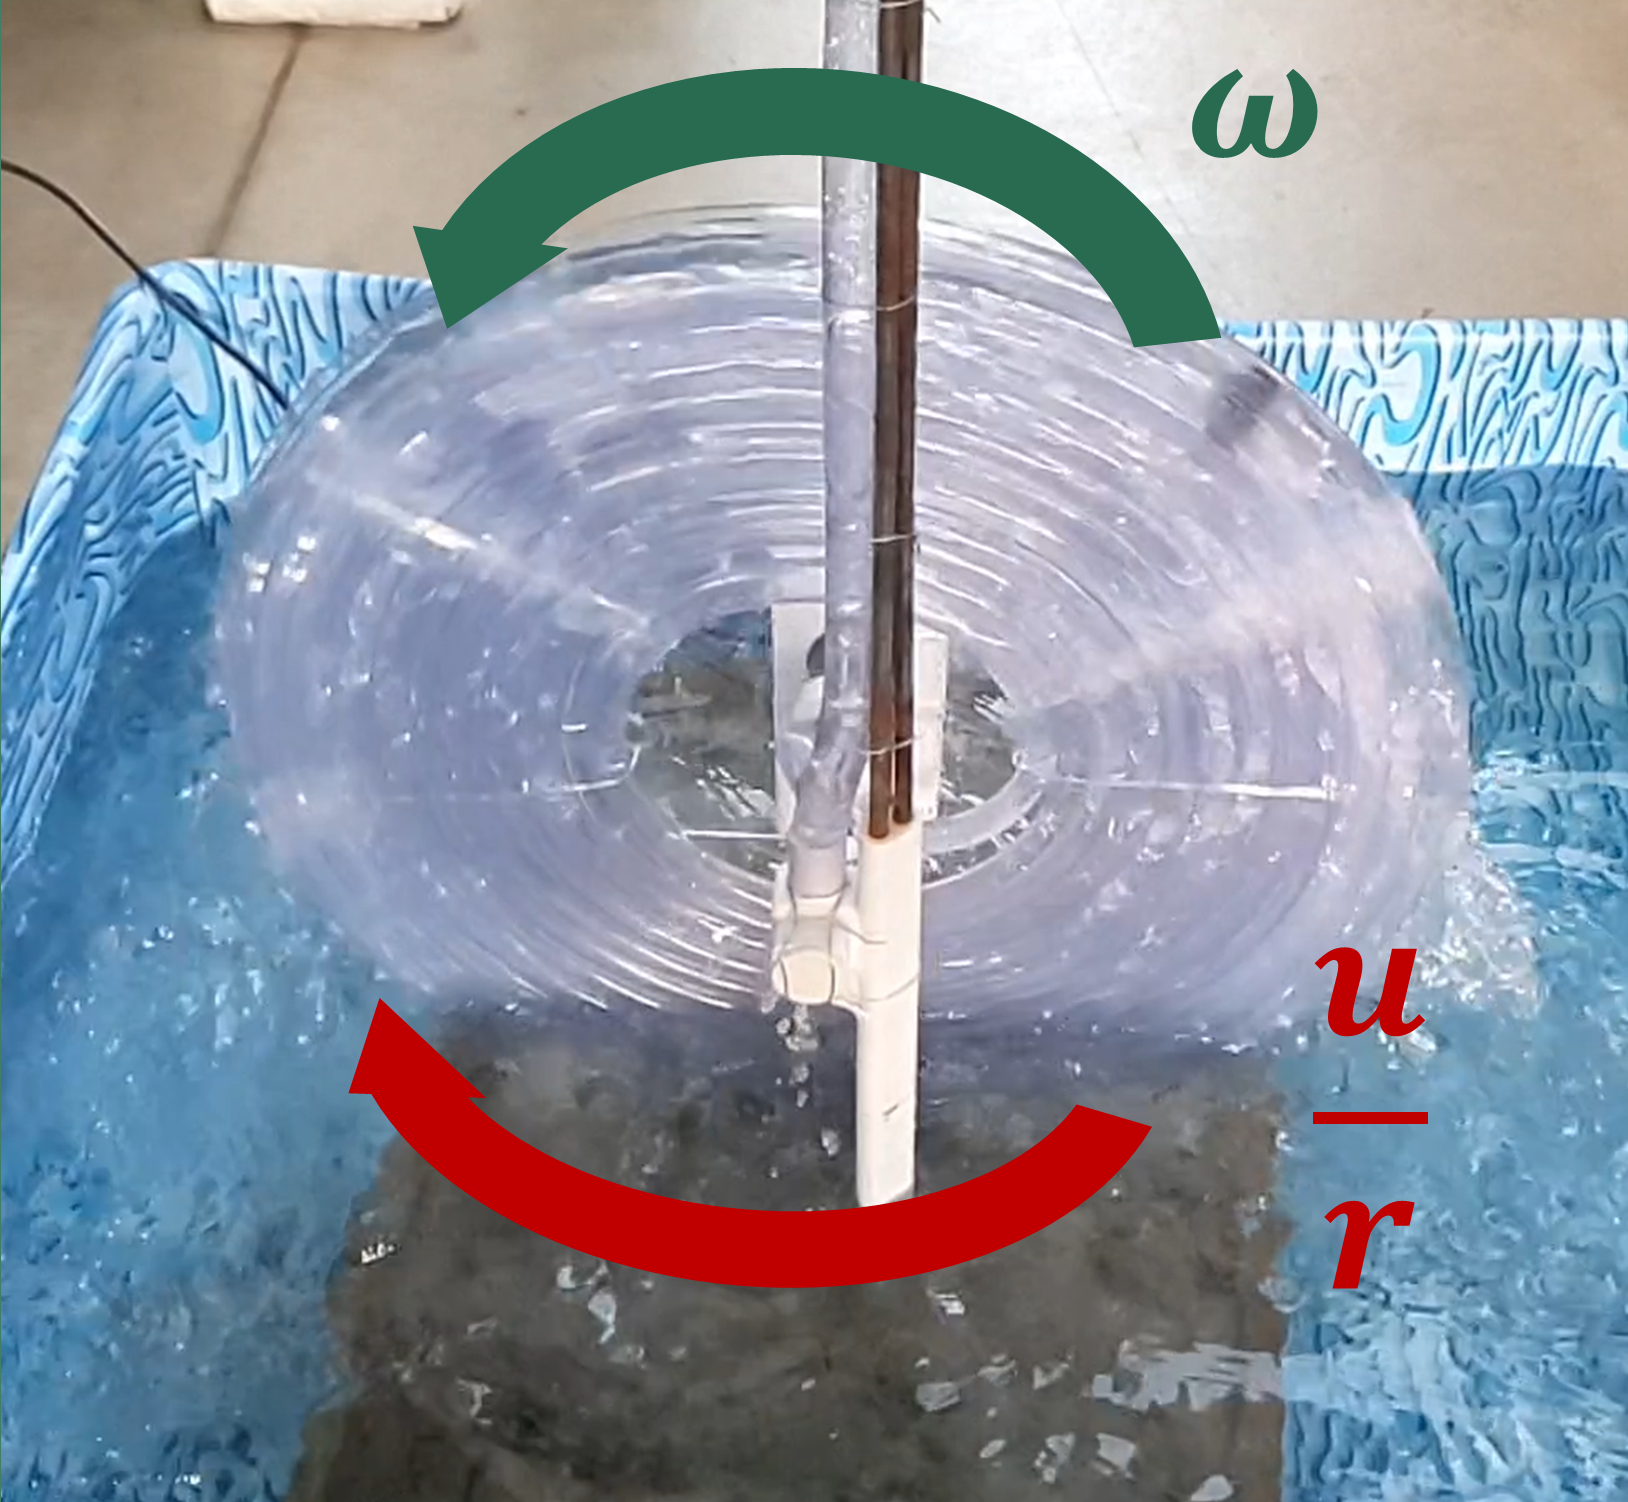
\includegraphics[width=\linewidth]{frame_velocity.png}\caption{}\end{subfigure}\hfill
  \begin{subfigure}[b]{0.49\columnwidth}\centering
    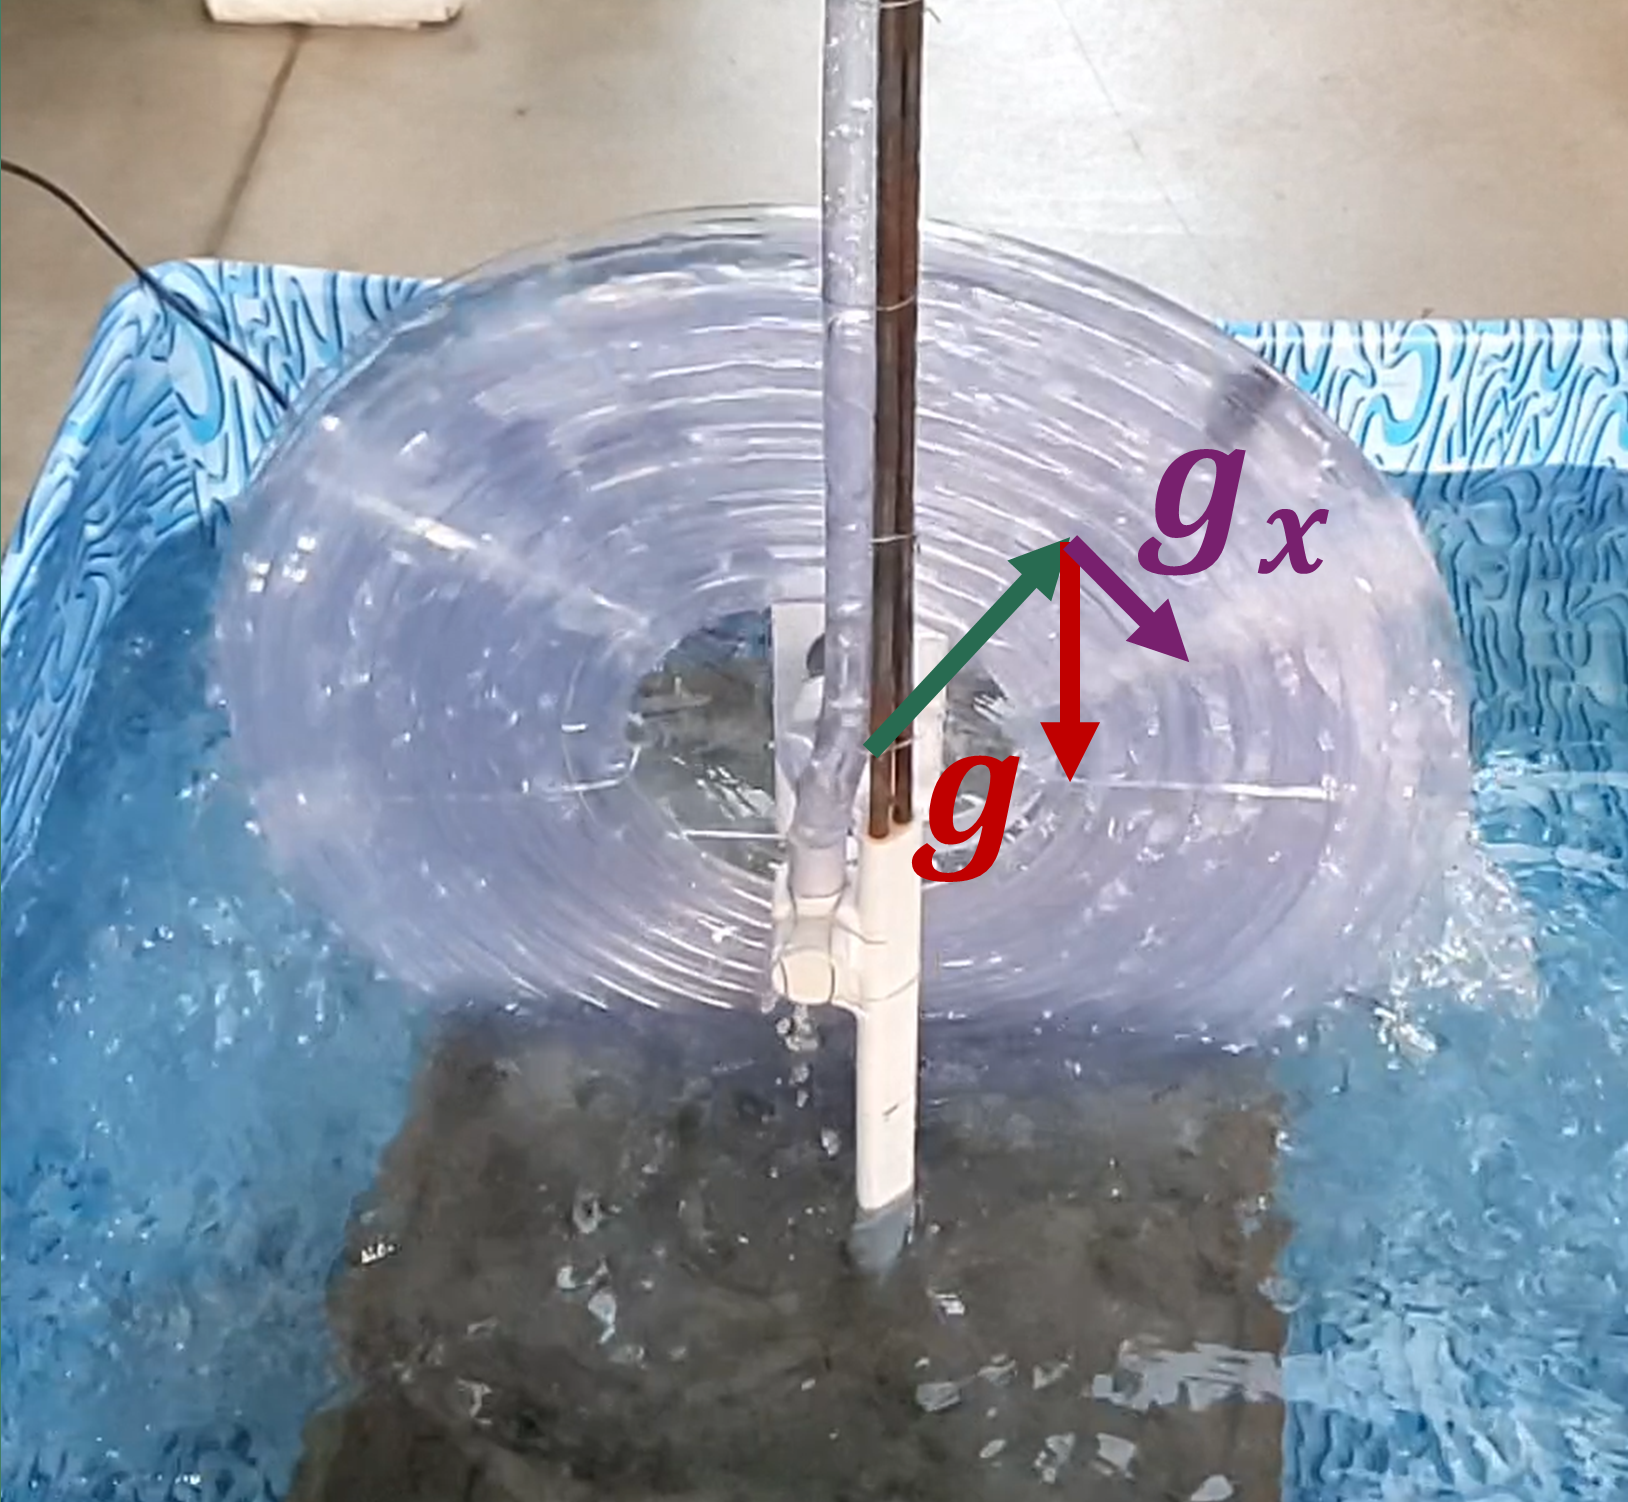
\includegraphics[width=\linewidth]{frame_gravity.png}\caption{}\end{subfigure}
  \caption{(a)~Enquanto a espiral gira a $\omega$, os tampões de água permanecem praticamente em repouso no laboratório e se movem a $w\simeq\omega r$ em relação ao tubo. (b)~Componente $g_x$ da gravidade ao longo do tubo.}
  \label{fig:frames}
\end{figure}

\subsection{Avaliação termo a termo}

\paragraph*{(i) Termo centrífugo.} Derivando a Eq.~\eqref{eq:param_phi} em relação a $x$,
\begin{equation}
  \frac{\partial\Phi_c}{\partial x} = \frac{\partial}{\partial x}\left(\tfrac12\omega^2r^2\right)
  = \omega^2r\,\frac{dr}{dx} = -\frac{\omega^2\varepsilon}{2\pi} .
  \label{eq:dphidx}
\end{equation}
O potencial centrífugo decresce \emph{linearmente} ao longo do tubo: a força centrífuga axial por unidade de massa é uniforme, igual a $\omega^2\varepsilon/2\pi$ e dirigida para fora. Como o integrando é constante, cada média de fase é a fração volumétrica correspondente vezes a constante, $\avg{\partial_x\Phi_c}=-\bm\alpha\,\omega^2\varepsilon/2\pi$, e o termo centrífugo da Eq.~\eqref{eq:averaged} vale
\begin{equation}
  \bm\rho\avg{\partial_x\Phi_c}L = -\,\bar\rho\,\frac{\omega^2\varepsilon L}{2\pi} = -\,\bar\rho\,\tfrac12\omega^2R_o^2 ,
  \label{eq:term_c}
\end{equation}
usando $L=\pi R_o^2/\varepsilon$, da Eq.~\eqref{eq:xtheta}.

\paragraph*{(ii) Termo inercial.} Da Eq.~\eqref{eq:param_w},
\begin{equation}
  \frac{\partial w}{\partial x} = -\frac{\omega}{2}\sqrt{\frac{\varepsilon}{\pi}}\,(L-x)^{-1/2} = -\frac{\omega\varepsilon}{2\pi r},
  \qquad
  w\frac{\partial w}{\partial x} = -\frac{\omega^2\varepsilon}{2\pi},
  \label{eq:dwdx}
\end{equation}
e o termo inercial, $\int_0^L w\,\partial_xw\,dx=\tfrac12 w^2\big|_0^L$, vale
\begin{equation}
  -\bm\rho\avg{w\,\partial_xw}L = +\,\bar\rho\,\frac{\omega^2\varepsilon L}{2\pi} = +\,\bar\rho\,\tfrac12\omega^2R_o^2 .
  \label{eq:term_i}
\end{equation}
Este é o ganho de pressão ``inercial'' $\omega^2\varepsilon L/2\pi$ que se obtém quando o balanço é escrito no referencial da espiral sem a força centrífuga. As Eqs.~\eqref{eq:dphidx} e \eqref{eq:dwdx} mostram que ele é cancelado \emph{ponto a ponto}, e não apenas na média:
\begin{equation}
  \frac{\partial\Phi_c}{\partial x} - w\frac{\partial w}{\partial x}
  = \frac{\partial}{\partial x}\left(\tfrac12\omega^2r^2-\tfrac12w^2\right) \equiv 0 ,
  \label{eq:bernoulli0}
\end{equation}
para cada uma das fases, isto é, para cada componente de $\mathbf I$. A Eq.~\eqref{eq:bernoulli0} é o invariante de Bernoulli no referencial em rotação: um elemento de fluido em repouso no laboratório tem $\tfrac12w^2-\tfrac12\omega^2r^2=0$ em todos os raios.

O cancelamento não é trivial. A força centrífuga é quase perpendicular ao tubo, reduzida pelo fator $|dr/dx|=\varepsilon/2\pi r$, mas é conservativa, e seu trabalho entre a entrada e o centro é $\tfrac12\omega^2R_o^2$ por unidade de massa, acumulado ao longo de muitas voltas. O termo cinético é reduzido pelo mesmo fator geométrico, Eq.~\eqref{eq:dwdx}, e os dois devem ser mantidos ou desprezados juntos. A mesma conclusão é obtida diretamente no referencial do laboratório, no qual os tampões estão (quase) em repouso e não há força centrífuga nem termo cinético a cancelar.

Com a geometria exata, o tubo cruza cada círculo sob o ângulo de passo $\alpha$ da Eq.~\eqref{eq:pitch}, a velocidade relativa é $w=\omega r\cos\alpha$, e o tampão deriva para o centro, no laboratório, com velocidade $\omega r\sin\alpha\simeq\omega\varepsilon/2\pi$, um passo por revolução. O invariante passa a ser
\begin{equation}
  \tfrac12\omega^2r^2 - \tfrac12 w^2 = \tfrac12\omega^2r^2\sin^2\alpha
  = \frac{\omega^2}{2}\left(\frac{\varepsilon}{2\pi}\right)^2\frac{\theta^2}{1+\theta^2},
  \label{eq:bernoulli}
\end{equation}
cuja variação ao longo de todo o tubo é limitada por $\omega^2\varepsilon^2/8\pi^2$: um resíduo de, no máximo, $\omega^2\varepsilon^2/(8\pi^2g)$ em altura.

\paragraph*{(iii) Termo viscoso axial.} Derivando novamente a Eq.~\eqref{eq:dwdx} com a Eq.~\eqref{eq:drdx},
\begin{equation}
  \frac{\partial^2 w}{\partial x^2} = \frac{\omega\varepsilon}{2\pi r^2}\frac{dr}{dx} = -\frac{\omega\varepsilon^2}{4\pi^2r^3}.
\end{equation}
Escrevendo a média de fase pela sua definição~\eqref{eq:avg}, a indicadora $I_w$ restringe a integral aos intervalos $[a_j,b_j]$ da Eq.~\eqref{eq:Iw}, e a média sobre a água se reduz a termos de fronteira nos meniscos,
\begin{align}
  \mu_wL\avg{\partial_x^2w}_w &= \mu_w\!\int_0^L I_w\,\partial_x^2w\,dx \nonumber\\
  &= \mu_w\sum_j\Big[\partial_xw\Big]_{a_j}^{b_j} \nonumber\\
  &= \mu_w\frac{\omega\varepsilon}{2\pi}\sum_j\left(\frac{1}{r(a_j)}-\frac{1}{r(b_j)}\right),
  \label{eq:term_v}
\end{align}
que, para um tampão curto, vale $-\mu_w\,\omega\varepsilon^2\ell/(4\pi^2r_j^3)$ por tampão. Em altura, isso corresponde a $\nu_w\omega\varepsilon^2\ell/(4\pi^2g\,r_j^3)\sim\SI{e-9}{m}$ para os valores representativos da Tabela~\ref{tab:terms}. Além disso, a Eq.~\eqref{eq:continuity} mostra que, para tampões rígidos, $\partial_xw=0$ e o termo se anula identicamente: a dissipação viscosa entra apenas pelo cisalhamento na parede.

\paragraph*{(iv) Termo gravitacional.} Este é o único termo que depende de \emph{onde} está a água. Com a Eq.~\eqref{eq:drdx}, a integral sobre o tampão $j$ tem a primitiva exata
\begin{align}
  \mathcal G_j &\equiv \int_{a_j}^{b_j} g\cos(\theta+\omega t)\,dx
  = \frac{g\varepsilon}{2\pi}\int_{\theta(b_j)}^{\theta(a_j)}\vartheta\cos(\vartheta+\omega t)\,d\vartheta \nonumber\\
  &= \frac{g\varepsilon}{2\pi}\Big[\mathcal F(\vartheta)\Big]_{\theta(b_j)}^{\theta(a_j)},
  \label{eq:Gj}
\end{align}
com
\begin{align}
  \mathcal F(\vartheta) &= \vartheta\sin(\vartheta+\omega t) + \cos(\vartheta+\omega t), \nonumber\\
  \mathcal F'(\vartheta) &= \vartheta\cos(\vartheta+\omega t).
  \label{eq:Fprim}
\end{align}
Como $\varepsilon\vartheta/2\pi=r$, temos $(g\varepsilon/2\pi)\mathcal F=g\,r\sin\phi+O(g\varepsilon)$, onde $r\sin\phi=z-z_a$ é a altura do ponto do tubo em relação ao eixo. A primitiva da gravidade é, portanto, a energia potencial, como deve ser para uma força conservativa: integrada sobre o tubo inteiro, ela fornece $\int_0^Lg_x\,dx=-gz_a$, independentemente da forma da espiral. Restrita a um tampão de comprimento $\ell$ centrado no ângulo de laboratório $\phi_j$, o tampão subtende $\Delta\vartheta=\ell/r_j$, e, como $\vartheta$ varia pouco nesse intervalo para $\theta\gg1$,
\begin{align}
  \mathcal G_j &\simeq g\,r_j\Big[\sin\!\big(\phi_j+\tfrac{\ell}{2r_j}\big)-\sin\!\big(\phi_j-\tfrac{\ell}{2r_j}\big)\Big] \nonumber\\
  &= 2g\,r_j\cos\phi_j\,\sin\frac{\ell}{2r_j} \equiv g\,\Delta z_j ,
  \label{eq:dz}
\end{align}
onde $\Delta z_j$ é o desnível entre o menisco do lado da entrada e o menisco do lado do centro. A dependência temporal de $g_x$ desaparece: os tampões estão em ângulos fixos $\phi_j$ no laboratório, e suas posições $\theta(a_j),\theta(b_j)$ no referencial da espiral recuam exatamente com $-\omega t$. O termo gravitacional da Eq.~\eqref{eq:averaged} é
\begin{align}
  \bm\rho\avg{g_x}L &= \rho_w\sum_j\mathcal G_j + \rho_a\!\int_0^L I_a\,g_x\,dx \nonumber\\
  &= \rho_w\,g\,\mathcal I(L,\varepsilon,d) + O(\rho_a),
  \label{eq:term_g}
\end{align}
com a integral gravitacional restrita à água,
\begin{equation}
  \mathcal I(L,\varepsilon,d) = \frac{\varepsilon}{2\pi}\sum_j\Big[\mathcal F(\vartheta)\Big]_{\theta(b_j)}^{\theta(a_j)}
  \simeq \sum_{j=1}^{N}2r_j\cos\phi_j\,\sin\frac{\ell}{2r_j},
  \label{eq:Ical}
\end{equation}
que depende da profundidade $d$ através do comprimento $\ell$ dos tampões.

\paragraph*{(v) Termo de parede.} A tensão na parede atua apenas sobre a água e, em termos do fator de atrito de Darcy $f$, vale $\tau_w=f\rho_ww^2/8$. Assim,
\begin{equation}
  \frac{4}{D}\avg{\tau_w}_wL = \rho_w g\sum_j\Delta H_{f,j}, \qquad
  \Delta H_{f,j} = f\,\frac{\ell}{D}\,\frac{w_j^2}{2g},
  \label{eq:term_w}
\end{equation}
a perda de carga de Darcy--Weisbach de cada tampão.

\paragraph*{(vi) Pressão e interfaces.} O lado esquerdo também se decompõe por fase. Como $I_w+I_a=1$, ele é a soma das médias de fase do gradiente de pressão; expandindo-as pela definição~\eqref{eq:avg} e usando a Eq.~\eqref{eq:Iw} --- que é o teorema~\eqref{eq:averaging_theorem} em uma dimensão, com as interfaces nos meniscos ---,
\begin{align}
  P(L)-P(0) &= L\sum_k\avg{\partial_xP}_k = \sum_k\int_0^L I_k\,\partial_xP\,dx \nonumber\\
  &= \sum_j\big[P\big]_{a_j}^{b_j} + \sum_{\text{bolsões}}\big[P\big]_{b_j}^{a_{j+1}} .
  \label{eq:sum}
\end{align}
Dentro de cada bolsão, $\partial_xP=\rho_ag_x\simeq0$: a pressão é uniforme, e o segundo somatório se anula. Os saltos capilares nos dois meniscos de um tampão são iguais e opostos e se cancelam em primeira ordem. Assim, as diferenças de pressão de todos os tampões se somam exatamente: os bolsões de ar são condutores ideais de pressão.

\subsection{A altura de bombeamento}

Substituindo os termos~(i)--(vi) na Eq.~\eqref{eq:averaged}, dividindo por $\rho_w$ e usando $P(L)-P(0)=\rho_wg(h-z_a)$ para a coluna no tubo de recalque, com $z_a$ a altura do eixo acima da superfície da piscina, obtemos a altura de bombeamento com todos os termos explícitos:
\begin{widetext}
\begin{equation}
  gh = gz_a
  \underbrace{+\;\frac{\bar\rho}{\rho_w}\,\frac{\omega^2\varepsilon L}{2\pi}}_{\text{inercial}}
  \underbrace{-\;\frac{\bar\rho}{\rho_w}\,\frac{\omega^2\varepsilon L}{2\pi}}_{\text{centrífugo}}
  \underbrace{+\;g\,\mathcal I(L,\varepsilon,d)}_{\text{gravitacional}}
  \underbrace{+\;\nu_w\frac{\omega\varepsilon}{2\pi}\sum_j\left(\frac{1}{r(a_j)}-\frac{1}{r(b_j)}\right)}_{\text{viscoso axial}}
  \underbrace{-\;g\sum_j\Delta H_{f,j}}_{\text{parede}}
  \;+\;O\!\left(\frac{\rho_a}{\rho_w}\right).
  \label{eq:height_full}
\end{equation}
\end{widetext}
A Tabela~\ref{tab:terms} compara a ordem de grandeza de cada termo, em metros de coluna d'água. Os termos inercial e centrífugo são individualmente comparáveis às alturas medidas, mas se cancelam exatamente, Eq.~\eqref{eq:bernoulli0}; o resíduo da geometria exata é milimétrico; o termo viscoso axial é nanométrico; e os termos do ar são reduzidos por $\rho_a/\rho_w\approx10^{-3}$. A perda na parede cresce com $\omega$, mas permanece subdominante na faixa medida (Sec.~\ref{sec:leak}). Por isso, e não por hipótese, o único termo que sobrevive é o gravitacional restrito à água:
\begin{equation}
  h = z_a + \mathcal I(L,\varepsilon,d) = z_a + \sum_{j=1}^{N}2r_j\cos\phi_j\,\sin\frac{\ell}{2r_j}.
  \label{eq:h_phi}
\end{equation}
A rotação não eleva a pressão diretamente; ela apenas transporta os tampões para as posições em que o seu peso sustenta a coluna.

\begin{table}[b]
  \caption{Ordem de grandeza dos termos da Eq.~\eqref{eq:height_full}, em altura de coluna d'água, para valores representativos $\varepsilon\approx\SI{2}{cm}$, $r\approx R_o\approx\SI{10}{cm}$, $\ell\approx\SI{10}{cm}$ e $\omega=\SI{450}{rpm}$.}
  \label{tab:terms}
  \begin{ruledtabular}
  \begin{tabular}{lcc}
    Termo & Expressão & Ordem (m) \\
    \midrule
    Inercial & $+\alpha_w\omega^2R_o^2/2g$ & $+0{,}5$ \\
    Centrífugo & $-\alpha_w\omega^2R_o^2/2g$ & $-0{,}5$ \\
    Resíduo de passo & $\le\omega^2\varepsilon^2/8\pi^2g$ & $10^{-3}$ \\
    Gravitacional & $\mathcal I(L,\varepsilon,d)$ & 0,1--2 \\
    Viscoso axial & $\nu_w\omega\varepsilon^2\ell/4\pi^2gr^3$ & $10^{-9}$ \\
    Termos do ar & $\times\rho_a/\rho_w$ & $10^{-3}$ relativo \\
  \end{tabular}
  \end{ruledtabular}
\end{table}

\paragraph*{O papel dos bolsões de ar.} A Eq.~\eqref{eq:h_phi} admite uma leitura complementar. Como a integral da gravidade sobre o tubo inteiro é $-gz_a$ e $I_w=1-I_a$, a Eq.~\eqref{eq:term_g} pode ser reescrita como
\begin{equation}
  h = -\frac1g\int_0^L I_a\,g_x\,dx = \sum_{\text{bolsões}}\Delta z^{(a)} ,
  \label{eq:airidentity}
\end{equation}
onde $\Delta z^{(a)}$ é o desnível vencido, ao longo do tubo, dentro de cada bolsão de ar. \emph{A altura de bombeamento é igual ao desnível total vencido pelos bolsões de ar.} A água sobe porque o ar, que não pesa, ``carrega'' o desnível; uma espiral cheia apenas de água ($\mathbf I=(1,0)^{\mathsf T}$) não bombeia.

\subsection{Altura de fechamento}

O ângulo $\phi_j$ da Eq.~\eqref{eq:h_phi} é a variável interna da bomba: a contrapressão empurra cada tampão pela lateral da volta até que o desnível equilibre a pressão. O desnível $\Delta z_j$ é máximo em $\phi_j=0$, com o tampão centrado no trecho vertical da volta; além disso, a água transborda para o bolsão de ar seguinte. A maior altura que a bomba pode sustentar, sua altura de fechamento, é portanto
\begin{equation}
  h_s = z_a + \sum_{j=1}^{N}2r_j\sin\frac{\ell}{2r_j} \;\simeq\; z_a + N\ell \qquad (\ell\ll r_j),
  \label{eq:hs}
\end{equation}
proporcional ao número de voltas.

\paragraph*{Dependência com a profundidade de imersão.} A entrada, no raio externo $R_o$, captura água enquanto está abaixo da superfície. Para uma imersão $d$, o eixo está a $z_a=R_o-d$ acima da superfície, e o arco submerso tem comprimento $\ell=2R_o\arccos(1-d/R_o)\simeq2\sqrt{2R_od}$ para $d\ll R_o$. Como a seção do tubo é constante e a água é incompressível, esse comprimento se conserva ao longo das voltas. Um tampão só se forma quando a entrada está imersa além de um limiar $d_0$, da ordem do diâmetro do tubo, abaixo do qual a água capturada não preenche a seção. Portanto,
\begin{equation}
  h_s(d) \simeq A_s\sqrt{d-d_0}, \qquad A_s = 2N\sqrt{2R_o},
  \label{eq:depth}
\end{equation}
e a altura de fechamento cresce com a raiz quadrada da profundidade. A altura do eixo $z_a=R_o-d$ da Eq.~\eqref{eq:hs} varia lentamente com $d$ em comparação com o termo $2N\sqrt{2R_od}$, cuja derivada é maior por um fator $N\sqrt{2R_o/d}\gg1$; um ajuste da Eq.~\eqref{eq:depth} absorve essa variação no limiar $d_0$, que é, portanto, um limiar efetivo e não puramente geométrico.

\paragraph*{Compressibilidade do ar.} Os bolsões são comprimidos isotermicamente à medida que a pressão cresce em direção ao centro, $P_j\ell_{a,j}=P_0\ell_{a,0}$. Para as maiores alturas medidas, $P/P_0\le1+\rho_wgh/P_0\approx1{,}21$, de modo que os bolsões encolhem no máximo cerca de 18\%. A compressibilidade é uma correção pequena na faixa medida, o que justifica o tratamento incompressível, mas ela limita bombas projetadas para alturas da ordem de \SI{10}{m}, em que os bolsões internos ficam reduzidos à metade.

\subsection{Refluxo e dependência com a rotação}
\label{sec:leak}

Como o ganho inercial está ausente, a rotação atua apenas através da vazão. Para alturas abaixo de $h_s$, a bomba entrega uma vazão proporcional a $\omega$, que diminui à medida que a contrapressão se aproxima da altura de fechamento. Adotamos a curva característica linear
\begin{equation}
  Q_p = q\,\frac{\omega}{2\pi}\left(1-\frac{h}{h_s}\right),
\end{equation}
onde $q$ é o volume de água capturado por revolução. A água também retorna através da bomba: o ar escorrega pelos tampões e a água escoa de volta ao longo da parede do tubo. Modelamos esse refluxo como proporcional à altura, $Q_\ell=k\,h$. No regime estacionário, a coluna de água está em repouso, de modo que $Q_p=Q_\ell$, e a altura de operação é a interseção da curva característica com a curva de refluxo:
\begin{equation}
  h = h_s\,\frac{\omega}{\omega+\omega_c}, \qquad \omega_c = \frac{2\pi k h_s}{q}.
  \label{eq:height}
\end{equation}
A altura cresce linearmente com a rotação para $\omega\ll\omega_c$ e satura na altura hidrostática de fechamento $h_s$, Eq.~\eqref{eq:hs}, na escala $\omega_c$ fixada pela razão entre refluxo e entrega. Combinando as Eqs.~\eqref{eq:depth} e \eqref{eq:height}, a $\omega$ fixo, obtém-se $h\propto\sqrt{d-d_0}$.

\paragraph*{Perdas na parede e rotação ótima.} O termo de parede da Eq.~\eqref{eq:height_full}, a perda de carga de Darcy--Weisbach $\Delta H_f=f(\ell/D)\,w^2/2g$ por tampão, com $w\simeq\omega r$, depende da rotação. No regime laminar, $f=64/\mathrm{Re}$ e a perda cresce linearmente com $\omega$; no regime turbulento, aproximadamente como $\omega^{7/4}$. Subtraída da Eq.~\eqref{eq:height}, ela produz um máximo de $h(\omega)$ seguido de uma queda: existe uma rotação ótima. A ausência de queda na faixa medida (Fig.~\ref{fig:h_omega}) mostra que essas perdas permanecem subdominantes até \SI{450}{rpm}, e por isso as desprezamos na análise dos dados.

%=====================================================================
\section{Resultados e discussão}
\label{sec:results}
%=====================================================================

A Figura~\ref{fig:h_omega} mostra a altura de bombeamento em função da rotação para os três tubos e para espirais com $N=4$ e $N=12$ voltas, junto com ajustes de mínimos quadrados da Eq.~\eqref{eq:height}. Os parâmetros ajustados estão na Tabela~\ref{tab:fits}. A Eq.~\eqref{eq:height} descreve as seis séries com desvio quadrático médio de 0,015--\SI{0.12}{m}, capturando tanto a subida inicial quanto a saturação da altura. Para o tubo~2 com $N=4$, a saturação ainda não é atingida na faixa medida, de modo que $h_s$ e $\omega_c$ são pouco determinados (grande $\omega_c$).

As alturas de fechamento das espirais com $N=12$ são 2,6--4,3 vezes as das espirais com $N=4$, próximas da razão entre os números de voltas, como esperado pela soma das alturas hidrostáticas, Eq.~\eqref{eq:hs}. A maior altura medida, \SI{2.2}{m}, é contada a partir da superfície da piscina; como o tubo de recalque começa no eixo de rotação, acima dessa superfície, ela ainda está dentro do tubo graduado de \SI{2}{m}.

\begin{figure}[t]
  \centering
  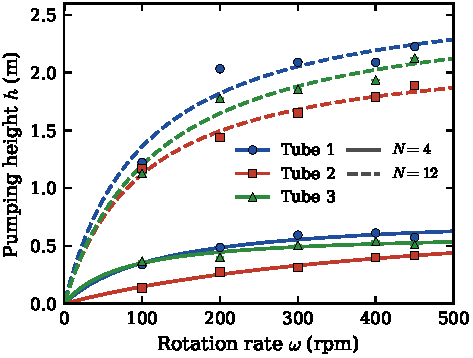
\includegraphics[width=\columnwidth]{height_vs_rpm_fit.pdf}
  \caption{Altura de bombeamento em função da rotação para os tubos~1--3 com $N=4$ (contínua) e $N=12$ (tracejada) voltas. Linhas: ajustes do modelo de refluxo, Eq.~\eqref{eq:height}; marcadores: experimento, com a incerteza de $\pm\SI{5}{rpm}$ em $\omega$.}
  \label{fig:h_omega}
\end{figure}

\begin{table}[b]
  \caption{Parâmetros das Eqs.~\eqref{eq:height} e \eqref{eq:depth} ajustados às medidas (incertezas: um desvio padrão do ajuste).}
  \label{tab:fits}
  \begin{ruledtabular}
  \begin{tabular}{lccc}
    \multicolumn{4}{l}{\emph{Séries em rotação, Eq.~\eqref{eq:height}}}\\
    Série & $h_s$ (m) & $\omega_c$ (rpm) & dqm (m) \\
    \midrule
    Tubo 1, $N=4$  & $0{,}78\pm0{,}07$ & $121\pm36$  & 0,027 \\
    Tubo 2, $N=4$  & $0{,}87\pm0{,}17$ & $492\pm164$ & 0,015 \\
    Tubo 3, $N=4$  & $0{,}61\pm0{,}05$ & $75\pm26$   & 0,025 \\
    Tubo 1, $N=12$ & $2{,}76\pm0{,}29$ & $103\pm39$  & 0,124 \\
    Tubo 2, $N=12$ & $2{,}24\pm0{,}10$ & $100\pm16$  & 0,043 \\
    Tubo 3, $N=12$ & $2{,}63\pm0{,}21$ & $119\pm32$  & 0,081 \\
    \midrule
    \multicolumn{4}{l}{\emph{Séries em profundidade ($N=4$), $h=A\sqrt{d-d_0}$}}\\
    Série & $A$ (m\,cm$^{-1/2}$) & $d_0$ (cm) & dqm (m) \\
    \midrule
    \SI{100}{rpm} & $0{,}373\pm0{,}015$ & $1{,}1\pm0{,}5$ & 0,085 \\
    \SI{200}{rpm} & $0{,}435\pm0{,}012$ & $1{,}5\pm0{,}3$ & 0,074 \\
    \SI{300}{rpm} & $0{,}314\pm0{,}008$ & $1{,}7\pm0{,}2$ & 0,055 \\
  \end{tabular}
  \end{ruledtabular}
\end{table}

A dependência com a profundidade de imersão é mostrada na Fig.~\ref{fig:h_depth} para três séries, cada uma tomada com um tubo diferente a uma rotação fixa. A lei em raiz quadrada $h\propto\sqrt{d-d_0}$, prevista pelas Eqs.~\eqref{eq:depth} e \eqref{eq:height}, descreve as três séries com desvio quadrático médio abaixo de \SI{0.09}{m}. Os limiares ajustados, $d_0\approx1$--\SI{2}{cm}, são da ordem dos diâmetros dos tubos, como antecipado. A amplitude $A=A_s\,\omega/(\omega+\omega_c)$ combina o fator geométrico $2N\sqrt{2R_o}$ com o fator de refluxo, de modo que não pode ser comparada diretamente entre séries tomadas com tubos diferentes. Como o fator de refluxo é menor que um, cada amplitude fornece, contudo, uma cota inferior para o raio externo, $R_o\geq\tfrac12(A/2N)^2$. Com $A$ convertida para unidades SI, os valores da Tabela~\ref{tab:fits} implicam $R_o\gtrsim8$--\SI{15}{cm}, uma verificação de consistência que pode ser confrontada diretamente com as dimensões do disco.

\begin{figure}[t]
  \centering
  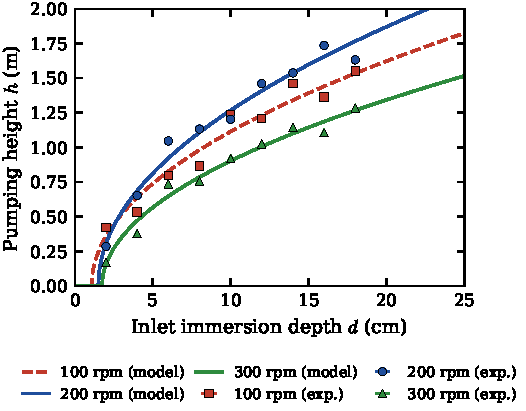
\includegraphics[width=\columnwidth]{height_vs_depth_fit.pdf}
  \caption{Altura de bombeamento em função da profundidade de imersão $d$ da entrada para três séries ($N=4$), cada uma com um tubo diferente na rotação indicada. Linhas: ajustes de $h=A\sqrt{d-d_0}$, Eqs.~\eqref{eq:depth} e \eqref{eq:height}; marcadores: experimento.}
  \label{fig:h_depth}
\end{figure}

%=====================================================================
\section{Conclusão}
\label{sec:conclusion}
%=====================================================================

A bomba de Wirtz eleva a água porque os bolsões de ar aprisionados entre os tampões transmitem, e somam, as diferenças de pressão produzidas pelos tampões inclinados em cada volta da espiral. Com funções indicadoras e o teorema da média espacial, mostramos que essas diferenças se somam exatamente e que a altura de bombeamento é igual ao desnível total vencido pelos bolsões de ar. Escrevendo a equação de Navier--Stokes do escoamento bifásico em notação matricial e avaliando cada termo da sua média volumétrica com a parametrização da espiral de Arquimedes, mostramos que o potencial centrífugo, de gradiente uniforme $-\omega^2\varepsilon/2\pi$, cancela ponto a ponto o termo inercial, um invariante de Bernoulli rotacional confirmado no referencial do laboratório; que o termo viscoso axial e os termos do ar são desprezíveis; e que a altura é, portanto, dada pela integral gravitacional restrita à água, para a qual obtivemos a primitiva exata. Ela é limitada por uma altura de fechamento proporcional ao número de voltas, que cresce com a raiz quadrada da profundidade de imersão, e reduzida pelo equilíbrio entre a entrega, proporcional à rotação, e o refluxo. A lei resultante, $h=h_s\,\omega/(\omega+\omega_c)$, reproduz a subida e a saturação da altura com a rotação, sua dependência em raiz quadrada com a profundidade de imersão e sua escala com o número de voltas. O modelo prevê ainda uma rotação ótima, além da faixa medida, acima da qual as perdas na parede passam a dominar.

\bibliography{references}

\end{document}
